\iflanguage{english}
{\chapter{Methoden und Umsetzung}}
{\chapter{Methods and Implementation}}
\label{sec:methods}
This chapter presents the methodology for estimating high-resolution full-body UV texture maps from a single RGB image. The overall system comprises two major pipelines. The first is the original SMPlitex\cite{casas2023smplitex} pipeline, as proposed by Casas and Comino-Trinidad, which employs a diffusion model conditioned on partial textures to synthesize complete $512 \times 512$ UV maps. The second is my extended pipeline, \ac{HRHumanTex}, which improves upon the baseline by introducing super-resolution data preparation, DreamBooth\cite{ruiz2023dreamboothfinetuningtexttoimage}-based fine-tuning, and high-resolution texture generation at $1024 \times 1024$. I will describe the construction of each pipeline in detail, support the description with flow diagrams and algorithm pseudocode, and provide comprehensive information on training settings, evaluation protocols, and implementation-specific challenges.

\section{SMPLitex Baseline Pipeline}

The SMPLitex pipeline estimates a full-body UV texture map from a single RGB image of a clothed person. Their method consists of three main stages: (1) estimating surface correspondences and silhouette masks, (2) constructing a partial UV texture, and (3) completing the texture using a diffusion model\cite{rombach2021highresolution} fine-tuned via DreamBooth. The output is a complete $512 \times 512$ UV texture $T_{\text{full}}$ compatible with the SMPL\cite{SMPL:2015} mesh. The overrall pipeline is showed in \ref{fig:smplitexpipeline}.


\begin{figure}[ht]
	\centering
	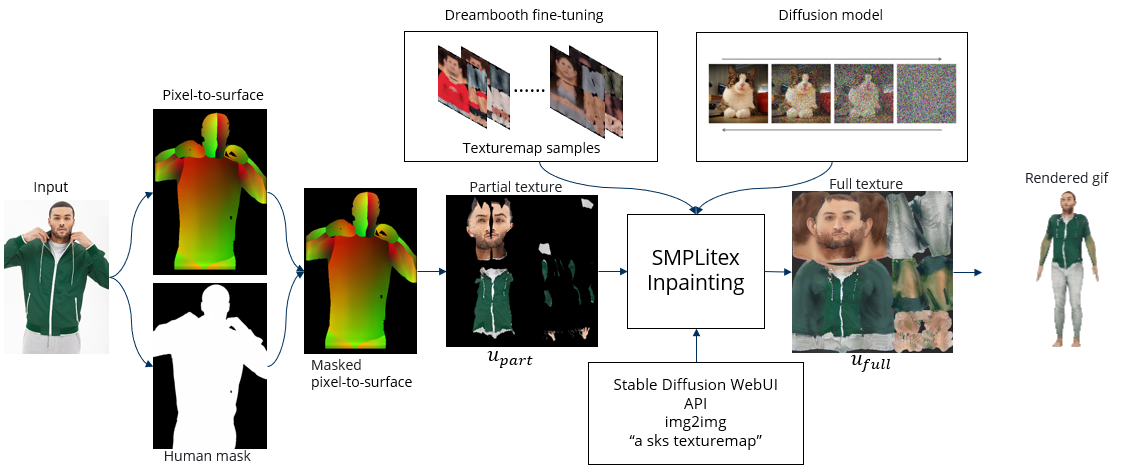
\includegraphics[width=1\textwidth]{fig/smplitex.png}
	\caption{SMPLitex human texturemap estimation
    pipeline}
	\label{fig:smplitexpipeline}
\end{figure}


\subsection{Pixel-to-Surface Mapping and Silhouette Extraction}

Given an input image $I$, SMPLitex first estimate a pixel-to-UV coordinate mapping using Densepose\cite{wu2019detectron2}. DensePose predicts, for each pixel $(x, y)$ in the image, the corresponding UV location $(u, v)$ on the SMPL surface. This defines the mapping $D(x, y) \rightarrow (u, v)$ for visible body pixels.

To prevent background pixels from contaminating the texture, they extract a high-quality foreground mask $M(x, y)$ using the  \cite{chen2022sghm}. \ac{SGHM} outputs a binary mask where $M(x, y) = 1$ indicates that pixel $(x, y)$ belongs to the human subject.

\subsection{Partial Texture Map Construction}

Using $D(x,y)$ and $M(x,y)$, they construct a partial UV texture $T \in \mathbb{R}^{512 \times 512 \times 3}$ and a visibility mask $T_m \in \{0,1\}^{512 \times 512}$:

\begin{algorithm}[H]
\caption{Partial UV Texture Projection}
\label{alg:smplitex_partial_texture}
\SetAlgoNlRelativeSize{0}
\SetKwComment{Comment}{$\triangleright$\ }{}
\DontPrintSemicolon
\KwIn{RGB image $I$, DensePose map $D(x, y)$, silhouette mask $M(x, y)$}
\KwOut{Partial texture $T$, mask $T_m$}
Initialize $T(u,v)\gets(0,0,0)$, $T_m(u,v)\gets 0$ for all $(u,v)$\;
\ForEach{pixel $(x,y)$ in $I$}{
    \If{$M(x,y) = 1$ and $D(x, y)$ is valid}{
        $(u,v) \gets D(x,y)$\;
        $(u',v') \gets (\lfloor u \cdot 511 \rfloor, \lfloor v \cdot 511 \rfloor)$\;
        $T(v', u') \gets I(y,x)$; \quad $T_m(v', u') \gets 1$\;
    }
}
\Return{$T, T_m$}
\end{algorithm}

This yields a partial texture $T$ where only front-facing (visible) parts of the subject are filled. The mask $T_m$ denotes the observed UV regions and is used in the inpainting step.

\subsection{Diffusion-Based Texture Completion}

To complete $T$, SMPLitex use a Stable Diffusion v1.4 model fine-tuned with DreamBooth on SMPL UV textures. Since only a limited number of example UV maps are available ($\sim$12), they employ \textbf{prior preservation} training with a learned token ``sks''. The model is trained using prompts like ``a sks texturemap'' (for instance data) and ``a texturemap'' (for general class prior). Training uses the following settings:

\begin{lstlisting}[language=bash]
accelerate launch --mixed_precision="fp16" train_dreambooth.py \
  --pretrained_model_name_or_path=CompVis/stable-diffusion-v1-4 \
  --instance_data_dir=./data_train \
  --output_dir=./smplitex-trained-model \
  --class_data_dir=./class_dir \
  --with_prior_preservation --prior_loss_weight=1.0 \
  --instance_prompt="a sks texturemap" \
  --class_prompt="a texturemap" \
  --resolution=512 \
  --train_batch_size=1 \
  --gradient_accumulation_steps=2 \
  --gradient_checkpointing \
  --learning_rate=1e-6 \
  --lr_scheduler="constant" \
  --lr_warmup_steps=0 \
  --num_class_images=10 \
  --max_train_steps=1500 \
  --checkpointing_steps=500 \
  --train_text_encoder \
  --use_8bit_adam
\end{lstlisting}

At inference, they load the fine-tuned model into the AUTOMATIC1111 WebUI~\cite{automatic1111webui} and use its API to perform masked inpainting. The input consists of $T$ (partial texture) and $T_m$ (mask), and the output is the full texture $T_{\text{full}}$.

\subsection{Key Components}
\subsection{DensePose-based Pixel-to-UV Mapping}
\label{sec:densepose}

To obtain pixel-to-surface correspondences between input RGB images and SMPL UV coordinates, we adopt DensePose~\cite{wu2019detectron2}, a widely used framework for dense human surface mapping. DensePose predicts, for each foreground pixel, its corresponding body part label $c$ and the local surface coordinates $(U, V)$ within that part.

The prediction process is formulated as a two-step mapping:
\begin{equation}
    c^{*} = \arg\max_{c} P(c \mid i), \quad [U, V] = R^{c^*}(i),
\end{equation}
where $P(c \mid i)$ is the predicted probability for each of the 24 SMPL body parts (plus background), and $R^{c^*}(i)$ is the regressor estimating the continuous UV coordinates for the selected part $c^*$.

To improve localization precision, DensePose adopts a region-based architecture similar to Mask R-CNN~\cite{matterport_maskrcnn_2017}, where region proposals are processed using RoIAlign~\cite{gong2021temporalroialignvideo} and passed through a dedicated FCN head to predict part labels and continuous coordinates. During training, a cross-entropy loss is used for part classification, and a Smooth-$L_1$ loss is used for the regression of UV coordinates.

Since only a sparse set of annotations (around 100--150 points per person), a distillation-based interpolation strategy is used. Specifically, a teacher network is trained to predict UV coordinates on labeled pixels and then deployed to infer dense pseudo-labels over the full foreground region.

This pixel-to-UV mapping enables the extraction of partial UV texture maps $\mathbf{u}_{\text{part}}$ from single-view input images,serving as a crucial component in many texture inpainting and reconstruction pipelines.


\subsection{Semantic-Guided Human Matting (SGHM)}
\label{sec:sghm}

SMPLitex adopts SGHM~\cite{chen2022sghm}, a high-quality human matting framework that uses semantic segmentation guidance to obtain accurate human silhouettes from a single image. The model is based on a multi-task architecture that shares a common encoder between segmentation and matting, enabling semantic features to inform detailed boundary enhancement.

Given an input image $I$, human matting aims to estimate the alpha matte $\alpha \in [0, 1]$ such that:
\begin{equation}
I = \alpha F + (1 - \alpha) B,
\end{equation}
where $F$ and $B$ are the foreground and background colors, respectively.

\paragraph{Shared Encoder.} SGHM shares the same encoder between segmentation and matting branches, built on ResNet-50~\cite{he2015deepresiduallearningimage} followed by an  Atrous Spatial Pyramid Pooling (ASPP)~\cite{chen2017rethinkingatrousconvolutionsemantic} module. It extracts multi-scale features $F_0, F_1, F_2, F_3, F_4$ from scales $\tfrac{1}{4}$ to $\tfrac{1}{64}$.

\paragraph{Segmentation Decoder.} A lightweight decoder progressively upsamples and merges encoder features to predict a coarse semantic mask $S$. Each layer follows:
\begin{equation}
X_i = \text{Conv}(\text{Concat}(\text{Upsample}(X_{i+1}), F_i)), \quad i = 3, 2, 1, 0.
\end{equation}

\paragraph{Matting Decoder.} To enhance the detail of the alpha matte, SGHM includes a dedicated matting decoder that focuses on uncertain boundary regions. It incorporates segmentation-aware features through an Attentive Shortcut Module (ASM), which fuses low-level encoder features and segmentation outputs using spectral normalization and channel-wise attention mechanisms. This enables the network to distinguish between subtle foreground-background transitions.

\paragraph{Progressive Refinement.} To generate high-resolution results, SGHM refines the predicted alpha map through a \textit{Progressive Refinement Module (PRM)}, which fuses alpha predictions across scales:
\begin{equation}
g_l = 
\begin{cases}
0 & \text{if } 0 < \alpha_{l-1} < 1 \\
1 & \text{otherwise}
\end{cases}
,\quad
\alpha_l = \alpha_l' g_l + \alpha_{l-1} (1 - g_l),
\end{equation}
where $\alpha_l'$ is the raw prediction at scale $l$ and $\alpha_{l-1}$ is the refined alpha from the previous scale.

This architecture enables SGHM to preserve confident regions while refining uncertain boundaries, producing fine-grained alpha mattes suitable for downstream compositing or texture extraction tasks.


\paragraph{Partial UV Texture.}
Using the DensePose mapping $D(x,y)$ and mask $M(x,y)$ from SGHM, visible colors are transferred to UV space. Each texel of the $512 \times 512$ UV map $T_{\text{part}}$ is filled by copying the pixel values from image $I$ whose UV coordinate matches the texel. A binary mask $T_m$ indicates which texels were observed.

\paragraph{Stable Diffusion and DreamBooth.}
SMPLitex uses a \ac{LDM}, specifically Stable Diffusion~\cite{rombach2021highresolution}, fine-tuned on texture maps. The model learns to complete the unobserved parts of $U_{\text{part}}$ by generating plausible patterns while preserving observed texels.

The inpainting model is trained using DreamBooth~\cite{ruiz2023dreamboothfinetuningtexttoimage}, a subject-specific fine-tuning method that preserves content by a class-specific prior loss. This ensures that textures remain semantically consistent and spatially aligned with human body structure.

During inference, $U_{\text{part}}$ is embedded into the \ac{LDM} latent space and completed via 20-step denoising using classifier-free guidance (CFG scale 2.0). The output is decoded and returned as the full texture $U_{\text{full}}$.


\subsection{Summary of SMPLitex Pipeline}

\begin{algorithm}[H]
\caption{SMPLitex Texture Estimation Pipeline}
\label{alg:smplitex_pipeline}
\SetAlgoNlRelativeSize{0}
\SetKwComment{Comment}{$\triangleright$\ }{}
\DontPrintSemicolon
\KwIn{Input image $I$}
\KwOut{Estimated full texture $T_{\text{full}}$}
Compute $D(x,y) \gets$ DensePose$(I)$ \Comment*[r]{pixel-to-UV mapping}
Compute $M(x,y) \gets$ SGHM$(I)$ \Comment*[r]{silhouette mask}
Project $T$, $T_m \gets$ \textsc{PartialTextureProjection}$(I, D, M)$ \;
Load DreamBooth-finetuned diffusion model \;
Inpaint using $T$, $T_m$ via Stable Diffusion \;
\Return $T_{\text{full}}$
\end{algorithm}

The resulting $T_{\text{full}}$ can then be applied to a SMPL mesh for rendering. This forms the baseline method that I extend in HRHumanTex.


\begin{figure}[ht]
	\centering
	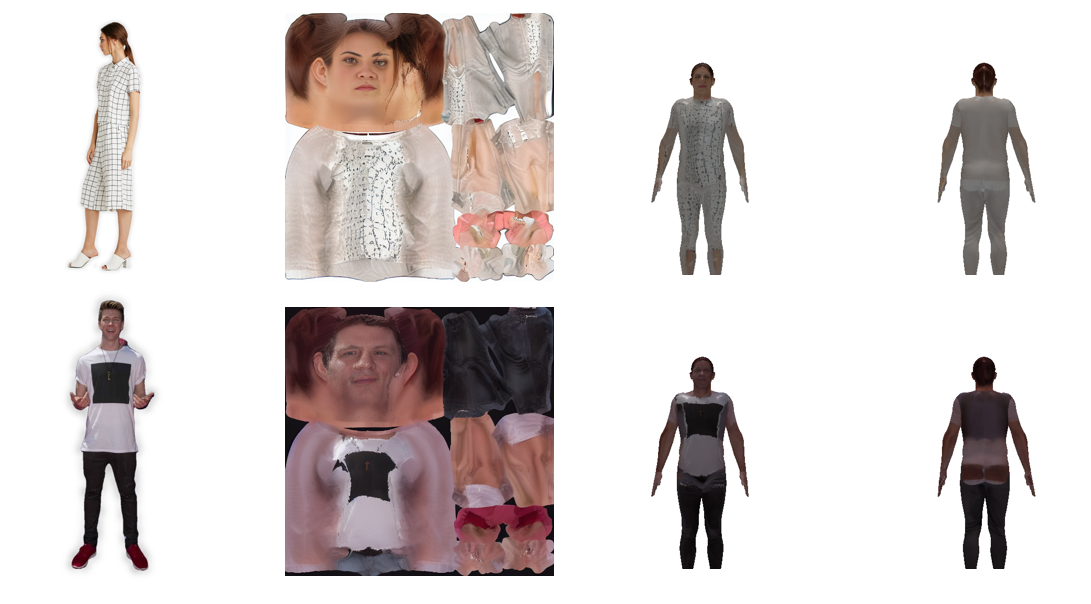
\includegraphics[width=0.9\textwidth]{fig/smplitex1.png}
     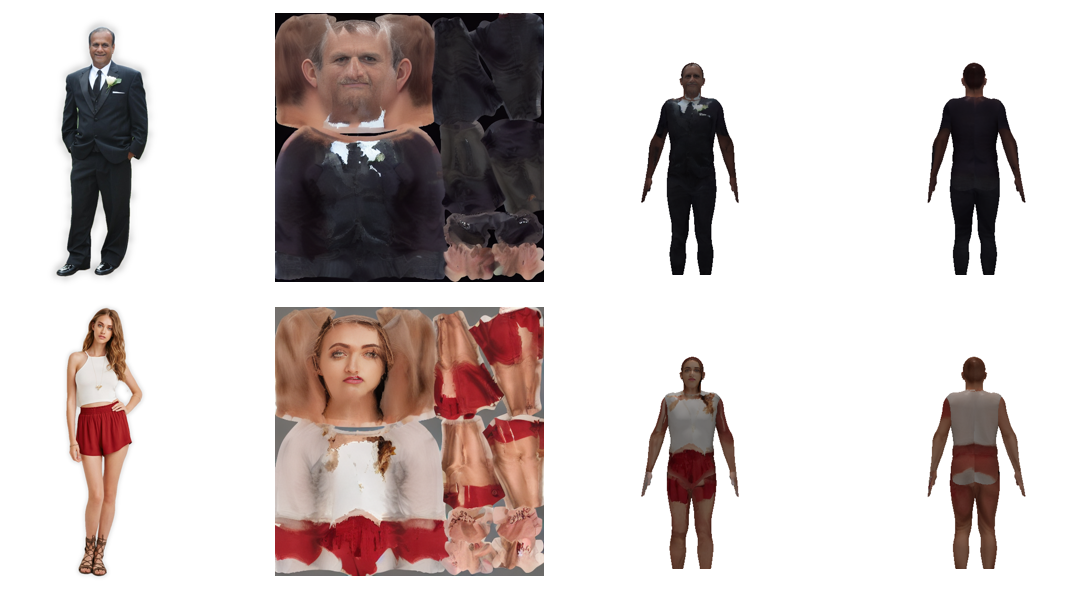
\includegraphics[width=0.9\textwidth]{fig/smplitex2.png}
	\caption{SMPLitex qualitative evaluation samples from dataset SHHQ~\cite{fu2022styleganhuman}.}
	\label{fig:smplitexeval}
\end{figure}

\section{HRHumanTex: Enhanced High-Resolution Pipeline and Evaluation Methodology}



\subsection{Limitations of the 512×512 Baseline Model}
The original SMPLitex texture based on DreamBooth fine-tuning at 512$^2$ resolution, suffers several limitations that motivate my high-resolution extension. First, it was trained on a small dataset (only $\sim$10–12 textures), which limits its ability to generalize. As a result, the baseline sometimes produces faulty or implausible textures for unseen clothing or patterns. More critically, the output resolution is restricted to 512×512, so fine details (high-definition logos, fabric weaves, etc.) are lost. If one attempts to directly use the 512px model at 1024px, the diffusion model yields severe artifacts. I observed it hallucinating content—for instance, generating ghostly facial features in regions of the UV map that do not correspond to a face. These aberrations occur because the base Stable Diffusion prior is biased toward producing face-like patterns, and without proper high-resolution training, it injects these into non-face areas. In short, the baseline model cannot natively produce coherent 1024×1024 textures, often producing distorted or repetitive details if forced to do so. These issues underscore the need for an improved pipeline, HRHumanTex, with dedicated high-resolution training to achieve realistic full-body textures at 1K resolution.


\subsection{Ablation Study A: Training Dataset Scale}
To determine the amount of training data needed for stable high-resolution texture synthesis, I conducted an ablation on dataset size. I first generated a pool of 266 high-resolution (1024×1024) UV textures by upscaling the available 512×512 ground-truth textures from SMPLitex dataset using RealESRGAN\cite{wang2021realesrgan} (a state-of-the-art GAN-based SR model). From this pool, I created training subsets of size 20, 50, 100, and the full 266, and fine-tuned separate 1024px models on each. 

Qualitatively, I found that very small training sets failed to cover the full body: with only 20 examples, the model largely reproduced only the central visible regions (e.g. front torso) and often left the side-body or limbs either blank or filled with muddled textures. With 50 examples, some improvement was seen, but the outputs were still inconsistent in completing peripheral regions like arms and back. Using 100 training textures markedly improved visual detail—the model began reliably generating plausible side-body and limb textures rather than just the center. Beyond 100, using all 266 samples yielded slightly more refined details but with diminishing returns. 

\begin{figure}[ht]
	\centering
	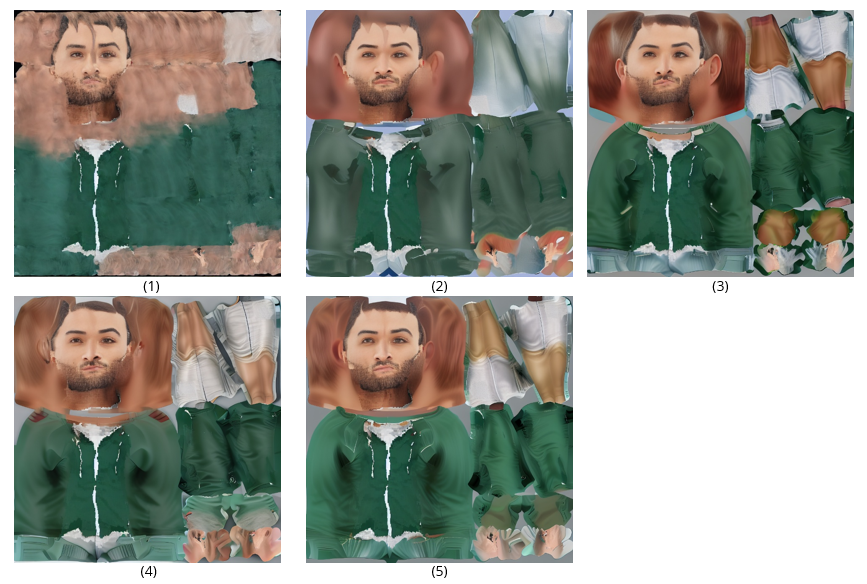
\includegraphics[width=1\textwidth]{fig/ablation1.png}
	\caption{Visual comparison of inpainting results using SMPLitex models trained on increasing dataset sizes. From left to right: (1) direct use of the original SMPLitex model without fine-tuning, (2) model trained on 20 textures, (3) model trained on 50 textures, (4) model trained on 100 textures, (5) model trained on 266 textures. Severe hallucinations are observed in the unfine-tuned model (1), especially in non-facial regions. With only 20 training samples, the model fails to generalize beyond frontal features. At 50 samples, the model begins to capture limbs and side-body areas. From 100 samples onward, full-body details become coherent, and the model trained on 266 textures produces the most consistent and high-fidelity result at 1024×1024 resolution. }
	\label{fig:Ablation1}
\end{figure}

\begin{figure}[ht]
	\centering
	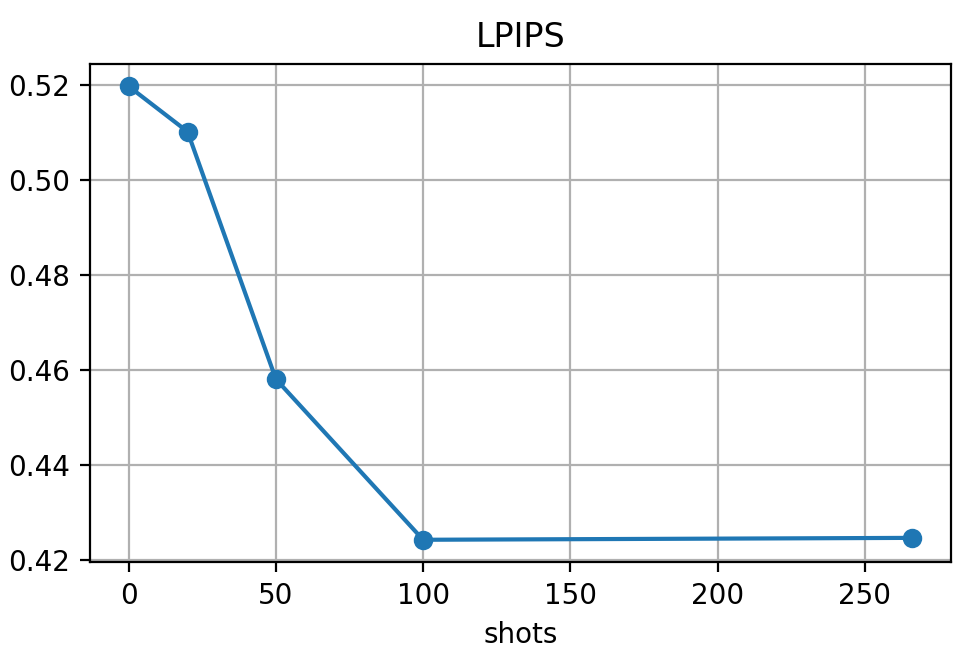
\includegraphics[width=0.5\textwidth]{fig/ablation1fig.png}
	\caption{Ablation study LPIPS metrics result.}
	\label{fig:Ablation1fig}
\end{figure}

The key observation is that at least on the order of \textbf{100+ high-resolution training examples} are required to achieve coherent full-body texture completion. Training on smaller subsets (20 or 50) led to models that would only correctly generate the most common details (typically the front torso area), whereas broader coverage of the body (consistent textures for arms, sides, and back) emerged only when the training dataset exceeded roughly one hundred examples. This data scalability experiment established that a large collection of diverse textures is essential for the diffusion model to generalize well to unseen people and poses at 1024×1024 resolution.



LPIPS~\ref{fig:Ablation1fig} more intuitively confirms my conclusions in the visual comparison.

\subsection{Super-Resolution(SR) Data Preparation and HRHumanTex Variants}
Simply gathering more real 1024px textures is difficult, so I leveraged image super-resolution to synthetically augment my training data. In particular, I experimented with seven modern \ac{SR} models to upscale the 512px ground-truth textures to 1024px: RCAN~\cite{zhang2018rcan}, Real-ESRGAN~\cite{wang2021realesrgan}, BSRGAN~\cite{zhang2021designing}, SwinIR~\cite{liang2021swinir}, DiffBIR~\cite{lin2024diffbir}, SRFormer~\cite{wang2024exploiting}. These cover a broad range of upsampling approaches— RCAN (Residual Channel Attention Network) is a traditional CNN-based SR model, Real-ESRGAN and BSRGAN are GAN-based methods for realistic detail enhancement, SwinIR and SRFormer are Transformer-based SR networks, and DiffBIR and StableSR employ diffusion models for resolution enhancement. 

Using each of these pre-trained SR models in turn, I upscaled all 266 available 512px UV textures to 1024px, yielding seven different high-resolution training sets (each with 266 images, one set per SR method). I then fine-tuned a separate DreamBooth model on each 1024px dataset, resulting in seven HRHumanTex variants labeled by the SR method used for data (e.g., \textit{HRHumanTex-266-RCAN}, \textit{-BSRGAN}, \textit{-SwinIR}, etc., alongside a \textit{-SRFormer} baseline). 

All variants were trained with identical settings to ensure a fair comparison. In particular, each used the same text conditioning (a fixed unique token representing “a sks texture map” concept), the same optimizer and hyperparameters (AdamW with learning rate $1\times10^{-6}$, no low-resolution warmup, and $\sim$2000 fine-tuning steps with prior-preservation regularization), and the same batch size (effectively 2 images per iteration via gradient accumulation). Training was done on an RTX3090 24GB GPU with gradient checkpointing and 8-bit weights to handle memory for 1024px; each model took roughly 7 hours to train (see Table\ref{tab:hrhumantex-variants} for a summary). By keeping the DreamBooth fine-tuning protocol constant across experiments, any differences in the output quality of these HRHumanTex variants can be attributed to the influence of the super-resolution preprocessing step. This allowed me to assess which SR-based data preparation leads to the best downstream texture generation.


\subsection{Two-Stage Upscaling Evaluation}

In order to identify the most effective Super-Resolution(SR) model to integrate into my pipeline, I carried out a two-stage evaluation on a held-out test set of textures. The evaluation aimed to measure: (1) which SR method best reconstructs a 512px texture from a lower-resolution input (simulating the diffusion model’s output stage), and (2) which SR method best produces 1024px textures from 512px inputs (for the final upsampling stage). Stage 1 can be evaluated against real ground-truth textures at 512px (since the dataset provides those), while Stage 2 lacks true 1024px ground truth—so I use the best method from Stage 1 to generate a high-quality pseudo-ground-truth for 1024px. 

The super-resolution methods used are summarized in Table~\ref{tab:sr_models}.

\begin{table}[t]
    \centering
    \caption{Summary of the $2\times$ super-resolution models considered, grouped by architectural class.}
    \label{tab:sr_models}
    \begin{tabular}{ll}
        \toprule
        \textbf{Model} & \textbf{Architecture Class} \\ 
        \midrule
        RCAN & CNN \\[2pt]
        Real-ESRGAN & GAN \\[2pt]
        BSRGAN & GAN \\[2pt]
        SwinIR & Transformer \\[2pt]
        SRFormer & Transformer \\[2pt]
        StableSR & Diffusion \\[2pt]
        DiffBIR & Diffusion \\ 
        \bottomrule
    \end{tabular}
\end{table}

\subsection{Inference Experiment Detail in Super-Resolution}
And this Table~\ref{tab:sr_inference_env} shows how I doing inference on 2x upscaling task.


\begin{table}[h]
\centering
\caption{Super-Resolution (SR) Models: Inference Environment and Configuration}
\label{tab:sr_inference_env}
\begin{tabular}{lccp{5cm}}
\toprule
\textbf{Model} & \textbf{Hardware} & \textbf{Resolution} & \textbf{Model Config / Checkpoint} \\
\midrule
\textbf{DiffBIR v2.1} & RTX 3090 (24GB) & $x2$ & Official release v2.1 \\
\textbf{StableSR} & RTX 3090 (24GB) & $x2$ & \texttt{stablesr\_000117.ckpt} \\
\textbf{SRFormer} & RTX 3090 (24GB) & $x2$ & \texttt{test\_SRFormer\_DF2Ksrx2.yml} \\
\textbf{RCAN} & RTX 3090 (24GB) & $x2$ & \texttt{RCAN\_BIX2.pt} \\
\textbf{SwinIR} & Google Colab (T4) & $x2$ & \texttt{003\_realSR\_BSRGAN\_DFO\_s64w8\_SwinIR-M\_x2\_GAN.pth} \\
\textbf{Real-ESRGAN} & Google Colab (T4) & $x2$ & \texttt{RealESRGAN\_x4plus} (default release) \\
\textbf{BSRGAN} & Google Colab (T4) & $x2$ & \texttt{BSRGANx2} from official repo \\
\bottomrule
\end{tabular}
\end{table}

\begin{algorithm}[t]
\caption{Evaluation Pipeline for High-Resolution Texture Upscaling}
\label{alg:eval_pipeline}
\SetAlgoNlRelativeSize{0}
\SetKwComment{Comment}{$\triangleright$\ }{}
\DontPrintSemicolon \KwIn{
Pre-trained SMPLitex diffusion model (512px output);\
Test set of textures with ground truth $T_{\text{gt}} \in \mathbb{R}^{512\times512\times3}$;\
Set of super-resolution models ${M_i}$ (including bicubic).
}
\KwOut{
Performance metrics (PSNR, SSIM, LPIPS, FID) for each SR model.
}
\BlankLine
\ForEach{test texture $T_{\text{gt}}$ in test set}{%
$T_{256} \leftarrow \text{Downsample}(T_{\text{gt}},256\times256)$ \Comment*[r]{Simulate low-res diffusion output}
\ForEach{SR model $M_i$}{%
$\hat{T}{512}^{(i)} \leftarrow M_i(T{256})$ \Comment*[r]{Upsample $256\to512$}
Compute PSNR, SSIM, LPIPS, FID between $\hat{T}{512}^{(i)}$ and $T{\text{gt}}$;
}%
}%
Select best SR model $M^{\ast}$ with highest PSNR/SSIM and lowest LPIPS/FID (Stage~1 winner);;
\BlankLine
\ForEach{test texture $T_{\text{gt}}$}{%
$T_{1024}^{\text{pseudo}} \leftarrow M^(T_{\text{gt}})$ \Comment*[r]{Upscale GT to 1024px as pseudo-GT}
\ForEach{other SR model $M_j$}{%
$\hat{T}{1024}^{(j)} \leftarrow M_j(T{\text{gt}})$ \Comment*[r]{Upsample $512\to1024$}
Compute PSNR, SSIM, LPIPS, FID between $\hat{T}{1024}^{(j)}$ and $T{1024}^{\text{pseudo}}$;
}%
}%
Aggregate metrics to identify best model for $512\to1024$ (Stage2 winner);;
\end{algorithm}


\textbf{Algorithm~\ref{alg:eval_pipeline}} summarizes this evaluation procedure. In Stage1, each ground-truth texture $T_{\text{gt}}$ (512×512) is downsampled to 256×256 to simulate a coarse output; then every candidate SR model $M_i$ (including a baseline bicubic scaler) upsamples it back to $512^2$. I compute fidelity metrics (PSNR, SSIM for distortion and LPIPS, FID for perceptual quality) between the SR result $\hat{T}_{512}^{(i)}$ and the original $T_{\text{gt}}$. 

The highest-performing model $M^*$ on these metrics is selected for the next stage. 

In Stage2, I use $M^{\ast}$ to upscale the \emph{ground-truth} 512px texture to 1024px,obtaining $T_{1024}^{\text{pseudo}}$ which serves as a reference “pseudo-GT.” Then, all other SR models $M_j{\ast}$ upscale the same 512px input to 1024px (producing $\hat{T}_{512}^{(i)}$), and I again compute metrics, this time against $T_{1024}^{\text{pseudo}}$. This reveals which method best preserves details at the $512\to1024$ upsampling step (by comparing each to the strong baseline $M^{\ast}$ output). Finally, I aggregate the results over the test set. 

\begin{figure}[ht]
	\centering
	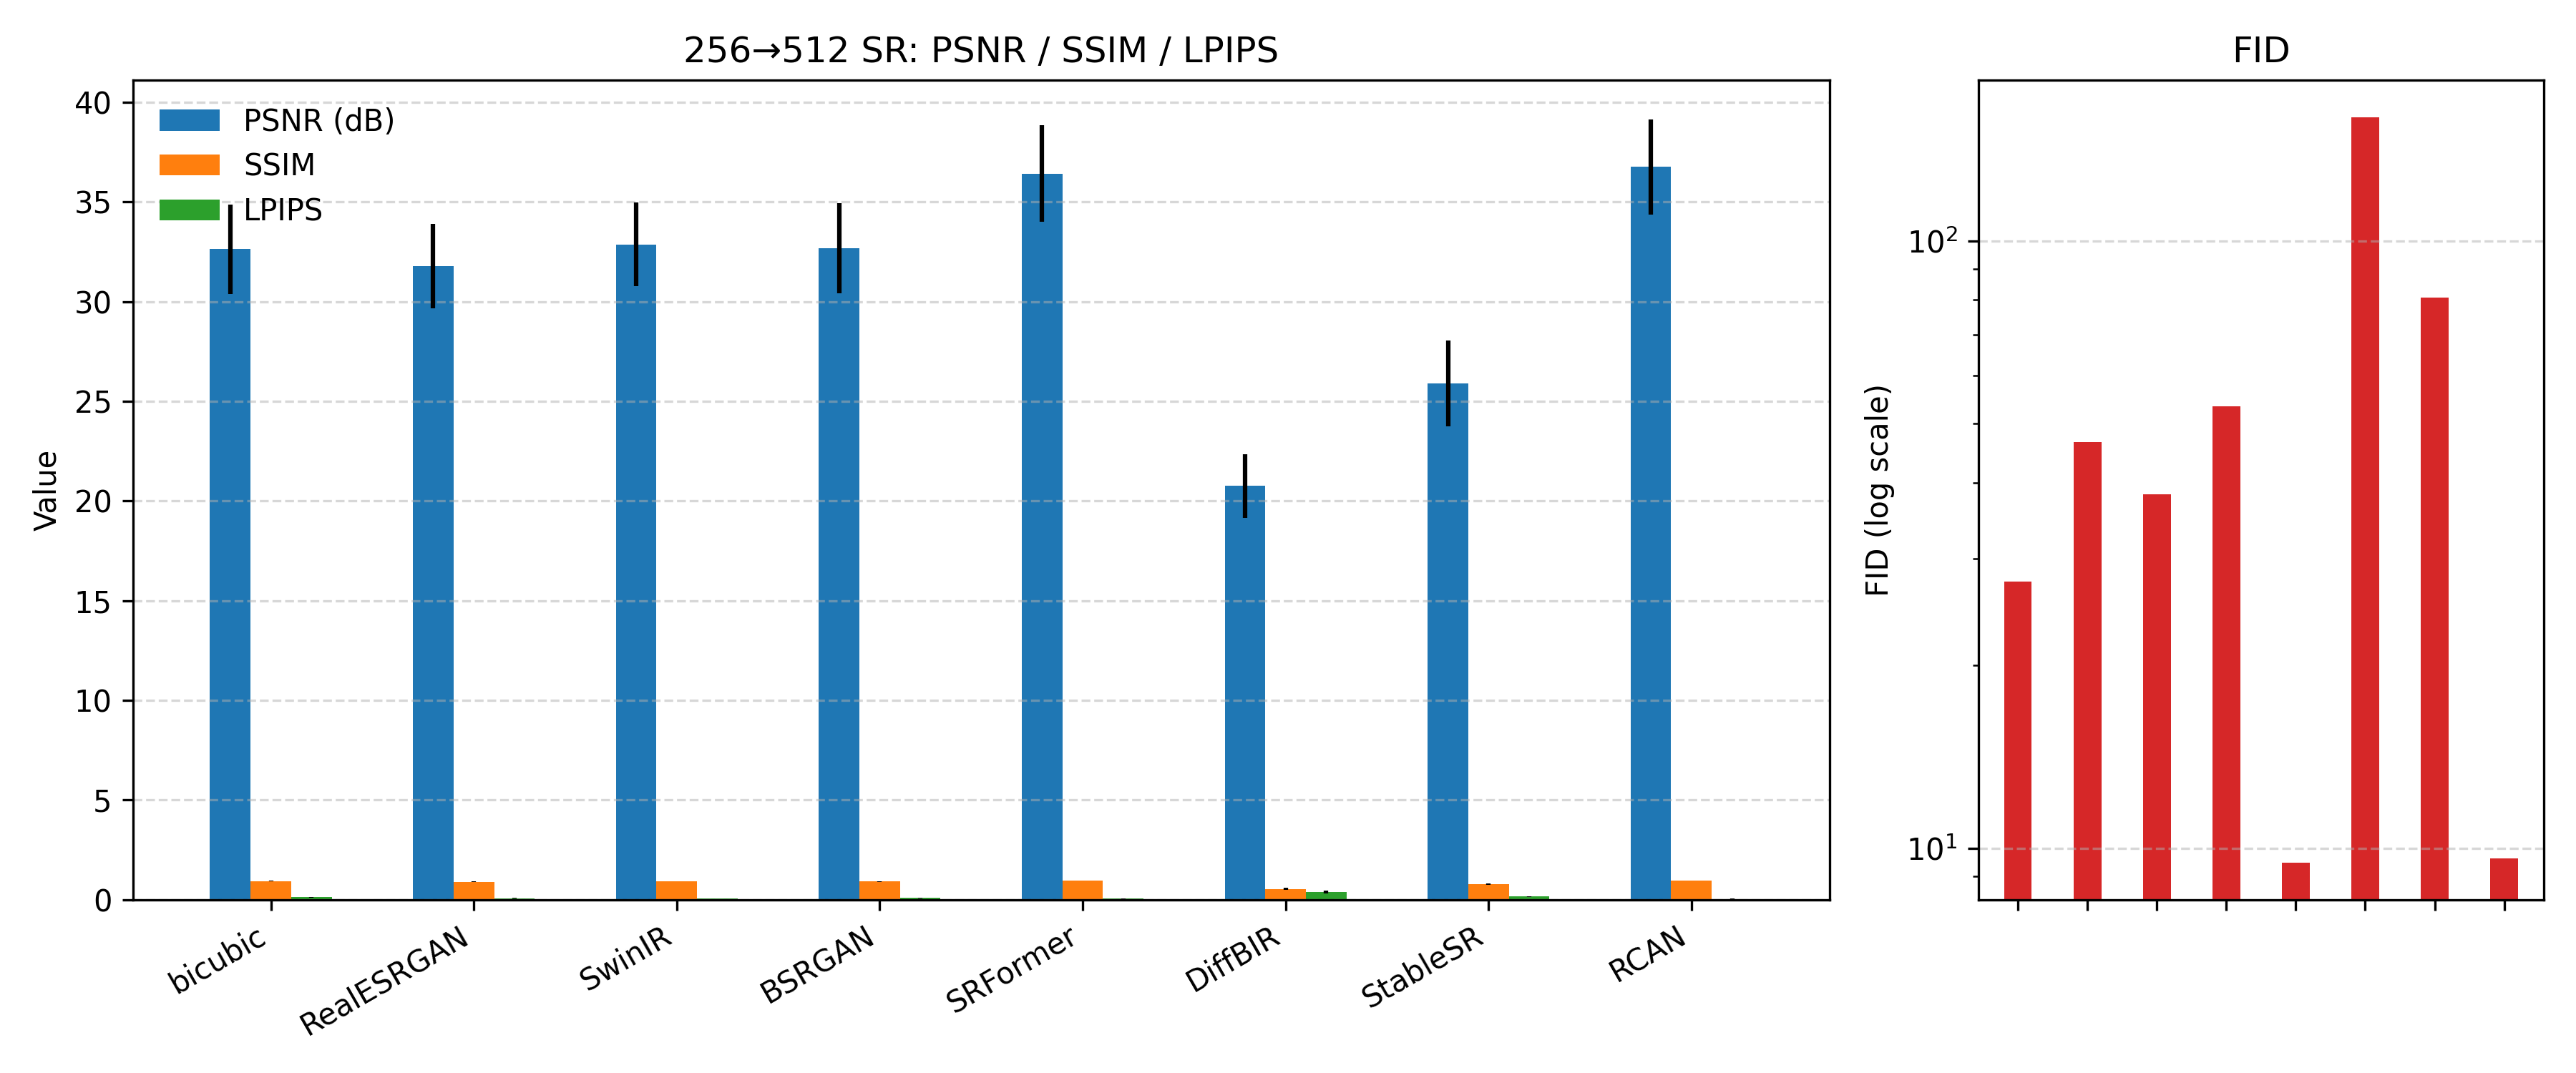
\includegraphics[width=1\textwidth]{fig/sr_256_512_comparison_twopanels.png}
	\caption{Quantitative evaluation panels on task 256→512 }
	\label{fig:256→512 panel}
\end{figure}



\begin{table}[t]
\centering
\caption{Quantitative results of 2$\times$ super-resolution models on task 256→512. Metrics are averaged over 50 test images.}
\label{tab:sr_metrics}
\begin{tabular}{lccccccc}
\toprule
\textbf{Model} & \textbf{PSNR}↑ & \textbf{SSIM}↑ & \textbf{LPIPS}↓ & \textbf{FID}↓ & \textbf{PSNR Std} & \textbf{SSIM Std} & \textbf{LPIPS Std} \\
\midrule
Bicubic     & 32.62 & 0.9412 & 0.1241 & 27.49 & 2.23 & 0.0137 & 0.0293 \\
Real-ESRGAN & 31.78 & 0.9067 & 0.0743 & 46.63 & 2.11 & 0.0152 & 0.0158 \\
SwinIR      & 32.86 & 0.9246 & 0.0634 & 38.24 & 2.10 & 0.0145 & 0.0147 \\
BSRGAN      & 32.67 & 0.9159 & 0.0890 & 53.39 & 2.27 & 0.0147 & 0.0220 \\
SRFormer    & 36.42 & \maxscore{0.9634} & 0.0496 & \maxscore{9.48}  & 2.41 & 0.0116 & 0.0213 \\
\minscore{DiffBIR}     & \minscore{20.75} & \minscore{0.5464} & \minscore{0.3984} & \minscore{159.70} & 1.61 & 0.0654 & 0.0791 \\
StableSR    & 25.90 & 0.7714 & 0.1571 & 80.71 & 2.15 & 0.0302 & 0.0245 \\
\maxscore{RCAN} & \maxscore{36.75} & \maxscore{0.9634} & \maxscore{0.0471} & 9.62  & 2.40 & 0.0115 & 0.0201 \\
\bottomrule
\end{tabular}
\end{table}



Using this rigorous procedure, I found that RCAN emerged as the top performer for 2× upscaling from 256→512 (Stage1). In fact, RCAN achieved a peak PSNR of about 36.75\,dB on my texture benchmark – noticeably higher than the next-best method (for example, SRFormer reached $\sim$36.42\,dB) – along with the highest SSIM (around 0.96) and lowest LPIPS. RCAN’s outputs were consistently sharper and more faithful to the original 512px textures, whereas GAN-based upscalers like Real-ESRGAN tended to introduce slight oversharpening or artifacts that lowered their fidelity scores. 


\begin{figure}[ht]
	\centering
	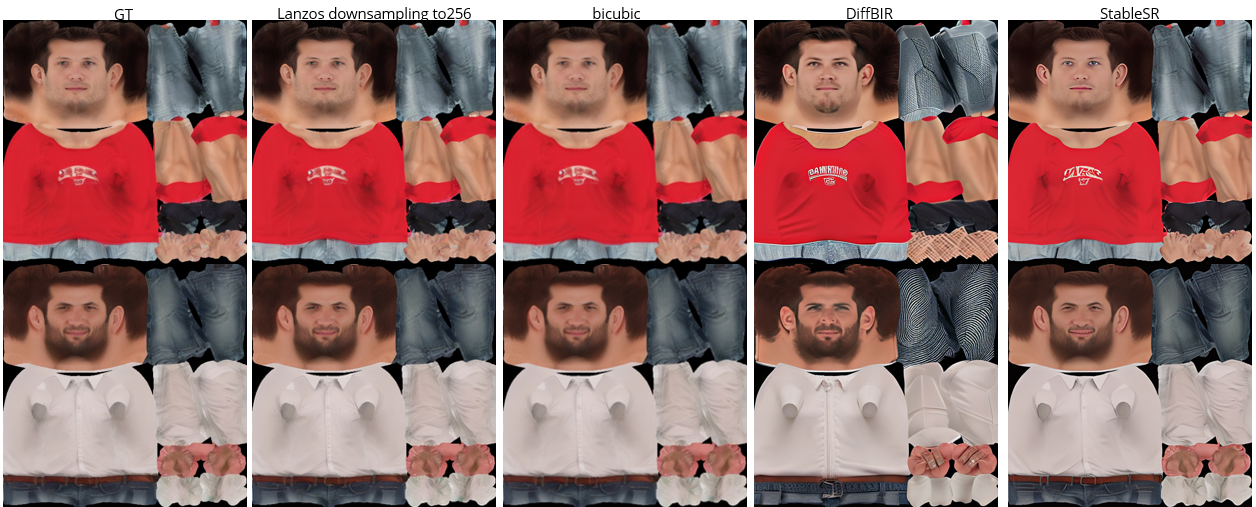
\includegraphics[width=1\textwidth]{fig/256-512_1.png}
        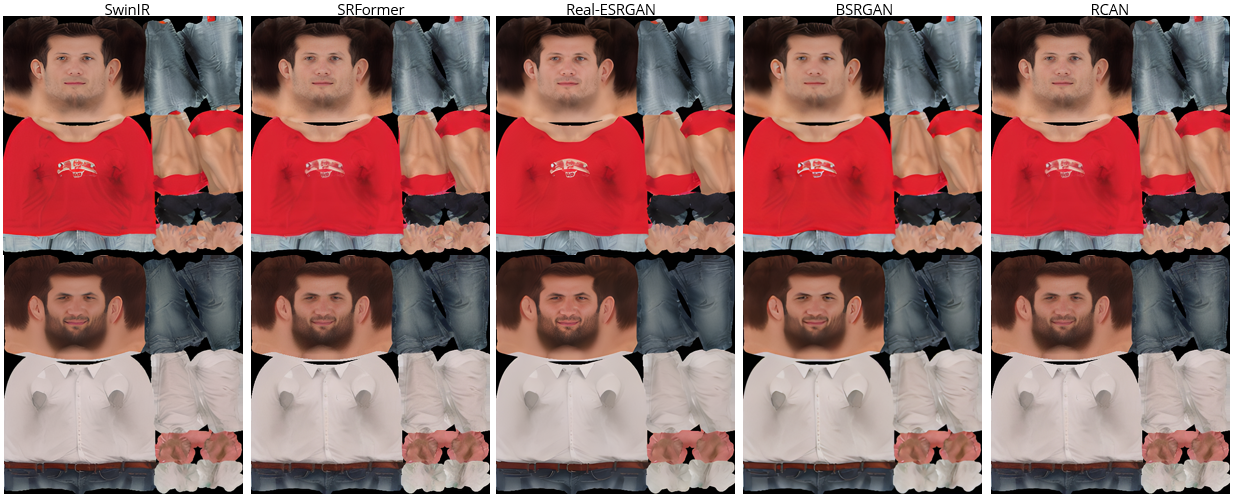
\includegraphics[width=1\textwidth]{fig/256-512_2.png}
	\caption{Visual comparison of 256→512 super resolution task on different \ac{SOTA} models }
	\label{fig:256→512 visual}
\end{figure}


Meanwhile, diffusion-based super-resolution models (i.e., DiffBIR and StableSR) performed notably worse. DiffBIR, in particular, had extremely poor performance across all metrics, with a PSNR below 21,dB and an FID score of 159.70, which is by far the worst across all models (see Table~\ref{tab:sr_metrics}). These results suggest that while diffusion models have strong generative capabilities, they may hallucinate overly complex or inconsistent patterns when applied to structured textures such as UV maps. 

This hypothesis is supported by qualitative results: in visual comparisons \ref{fig:256→512 visual}, both DiffBIR and StableSR produced outputs that contained excessive details or unnatural high-frequency noise—often inconsistent with the actual structure of the original texture. One possible reason is that diffusion models, by design, are trained to be creative under uncertainty; when applied to simple low-resolution textures, they may overinterpret the input and “imagine” details that do not exist. In contrast, transformer-based models such as SwinIR and SRFormer struck a balance between fidelity and perceptual sharpness, outperforming GANs in most metrics while preserving better global consistency. \ref{fig:256→512 face} show the detail comparison on of face region, 

\begin{figure}[ht]
	\centering
	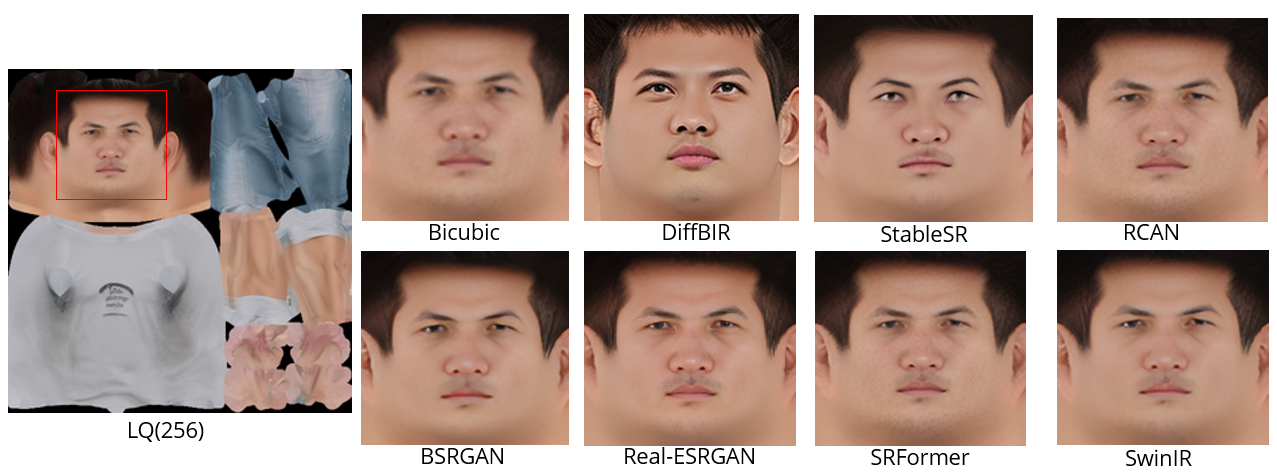
\includegraphics[width=1\textwidth]{fig/256-512_face.png}
        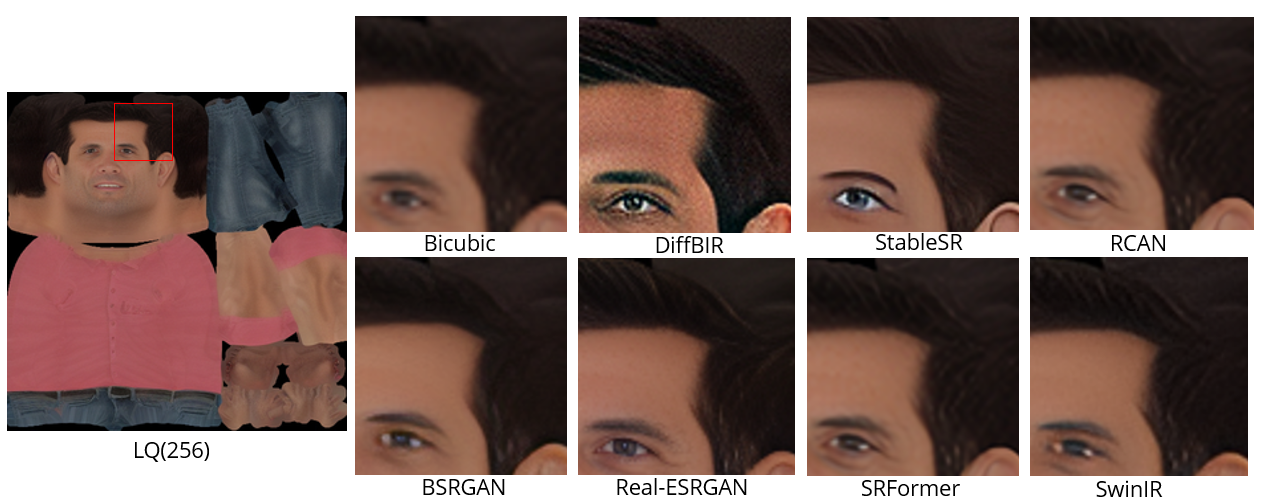
\includegraphics[width=1\textwidth]{fig/256-512_face2.png}
	\caption{Face region detail comparison of 256→512 super resolution task on different \ac{SOTA} models}
	\label{fig:256→512 face}
\end{figure}

\begin{table}[h]
\centering
\caption{Comparison of SR models for $512\rightarrow1024$ upsampling using RCAN outputs as pseudo-GT. Metrics are averaged over 50 samples.}
\label{tab:sr_eval_512_1024}
\begin{tabular}{lccccccc}
\toprule
\textbf{Model} & \textbf{PSNR}↑ & \textbf{PSNR Std} & \textbf{SSIM}↑ & \textbf{SSIM Std} & \textbf{LPIPS}↓ & \textbf{LPIPS Std} & \textbf{FID}↓ \\
\midrule
Bicubic       & 34.13 & 2.14 & 0.9645 & 0.0094 & 0.1041 & 0.0219 & 27.27 \\
Real-ESRGAN   & 32.24 & 1.61 & 0.9133 & 0.0143 & 0.1132 & 0.0243 & 39.96 \\
SwinIR        & 33.94 & 1.76 & 0.9381 & 0.0113 & 0.0804 & 0.0167 & 28.68 \\
BSRGAN        & 33.40 & 1.88 & 0.9202 & 0.0141 & 0.1105 & 0.0229 & 39.98 \\
\maxscore{SRFormer} & \maxscore{42.78} & 2.86 & \maxscore{0.9944} & \maxscore{0.0017} & \maxscore{0.0056} & \maxscore{0.0020} & \maxscore{1.69} \\
\minscore{DiffBIR}  & \minscore{24.53} & 1.94 & \minscore{0.6724} & \minscore{0.0437} & \minscore{0.3380} & \minscore{0.0568} & \minscore{100.00} \\
StableSR      & 27.73 & 2.13 & 0.8116 & 0.0274 & 0.1759 & 0.0251 & 63.65 \\
\bottomrule
\end{tabular}
\end{table}

\begin{figure}[ht]
	\centering
	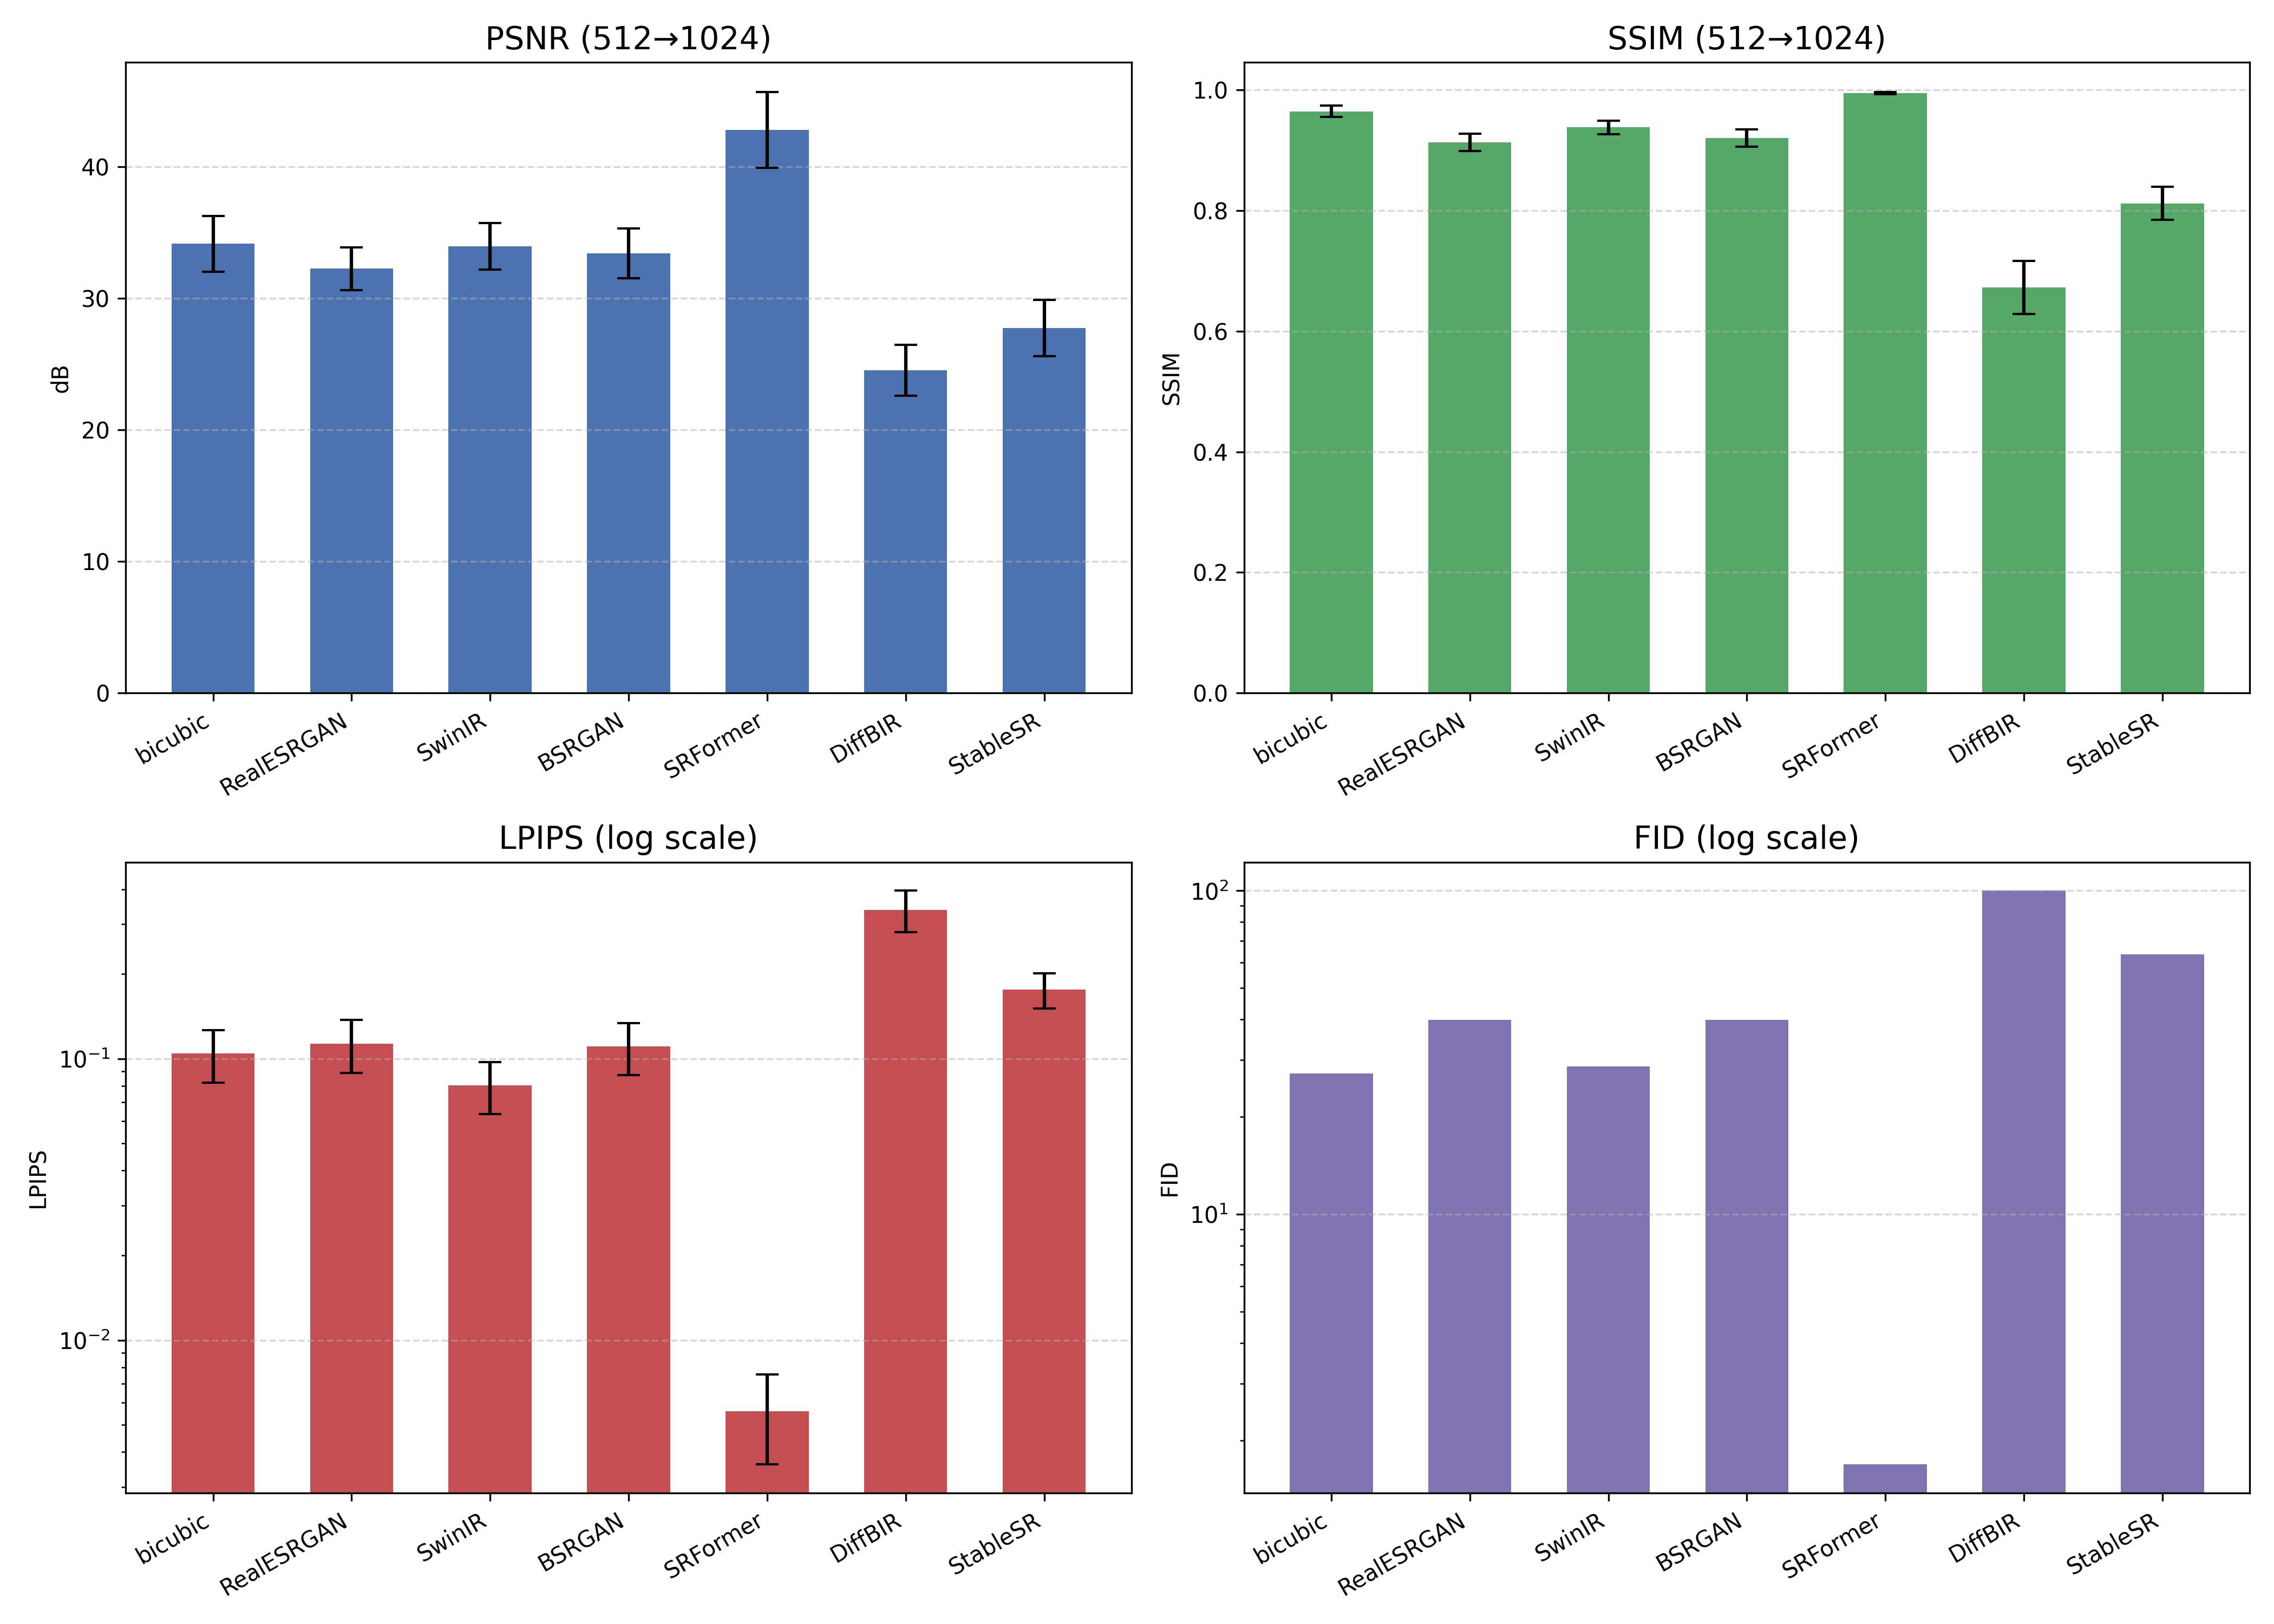
\includegraphics[width=1\textwidth]{fig/sr_512_1024_comparison.png}
	\caption{Quantitative evaluation of 512→1024 super resolution task on different \ac{SOTA} models}
	\label{fig:512→1024 fig}
\end{figure}





For the 2× upsampling from 512→1024 (Stage2), the evaluation against the RCAN-upscaled pseudo-GT indicated that SRFormer was marginally superior to the others. According Table~\ref{tab:sr_eval_512_1024}, SRFormer achieved the highest PSNR and the best structural similarity; its transformer-based architecture excelled at preserving fine details even when doubling an already high resolution. In summary, RCAN was identified as the best intermediate upsampler, and SRFormer as the best final-stage upsampler, according to these quantitative comparisons.


\subsection{Integrate Super-Resolution Module into HRHumanTex with Inpainting Evaluation}
After conducting two-stage super-resolution evaluation (256→512 and 512→1024), I proceed to a final inpainting-centered evaluation to determine which SR-generated dataset yields the most effective HRHumanTex model.

\paragraph{Step 1: Evaluation Setup.}
I begin by selecting 50 images from the DeepFashion~\cite{liuLQWTcvpr16DeepFashion} dataset. The selection emphasizes diversity in pose, clothing material, color, texture, and skin tone to ensure broad generalization. For each input photo:

\begin{enumerate}
\item I estimate the 3D body using SMPLitex to obtain a 512×512 texture.
\item I apply SRFormer to upscale this baseline texture to 1024×1024. This upscaled result is used as the pseudo-ground-truth.
\end{enumerate}

\paragraph{Step 2: Inpainting Model Comparison.}
Next, I run the same 50 inputs through each of the 7 HRHumanTex variants—each trained using a dataset upscaled by one of the 7 SR models (RCAN, BSRGAN, Real-ESRGAN, SwinIR, DiffBIR, SRFormer, StableSR). For each model, I generate a full $1024^2$ texture from the partial input. This yields 7 sets of predicted textures. Figure~\ref{fig:inpainteval1} shows visual comparison results. Table~\ref{tab:inpaint_eval1} shows traditional quantitative evaluation results.
\begin{figure}[ht]
	\centering
	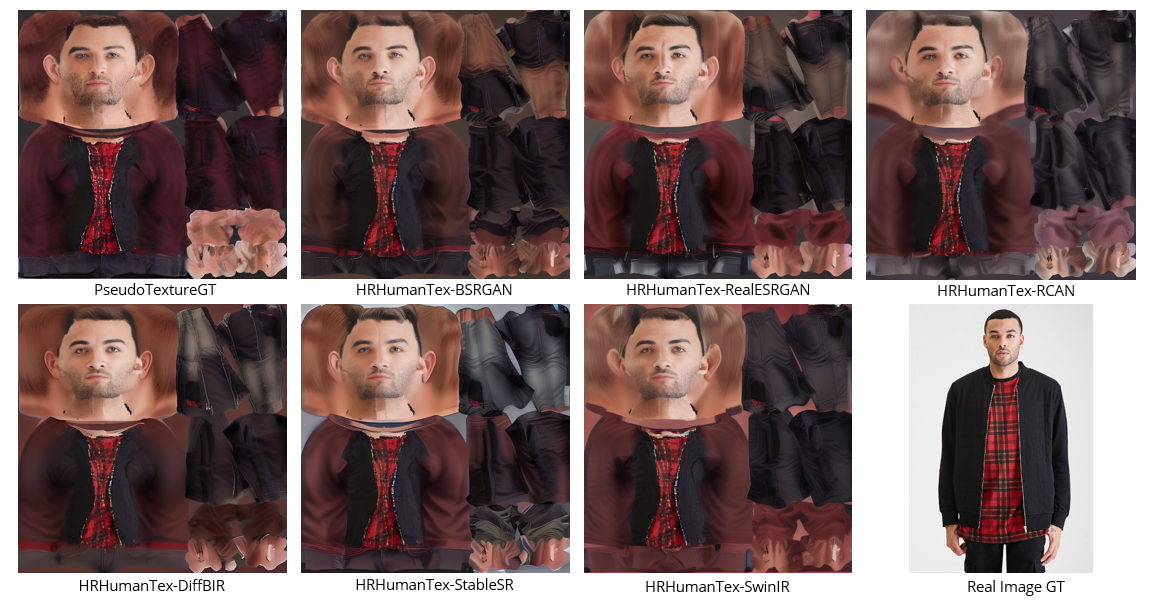
\includegraphics[width=1\textwidth]{fig/df1.png}
    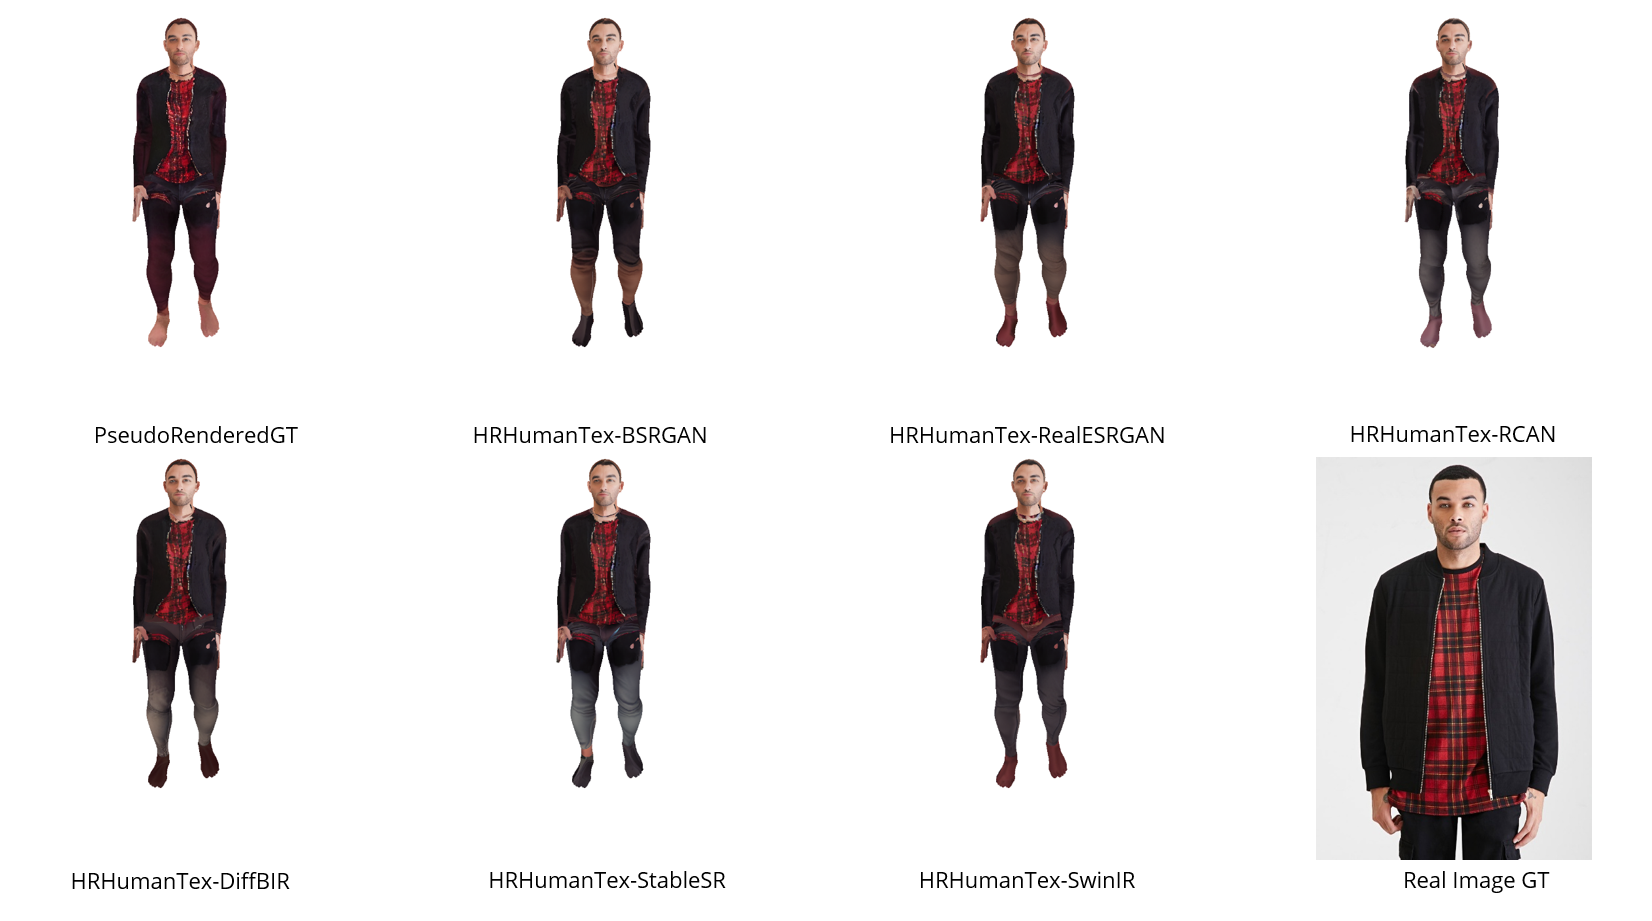
\includegraphics[width=1\textwidth]{fig/df2.png}
	\caption{Visual comparison of different inpainting models in UV space and rendered images, data sampled from dataset DeepFashion~\cite{liuLQWTcvpr16DeepFashion}.}
	\label{fig:inpainteval1}
\end{figure}

\begin{figure}[ht]
	\centering
	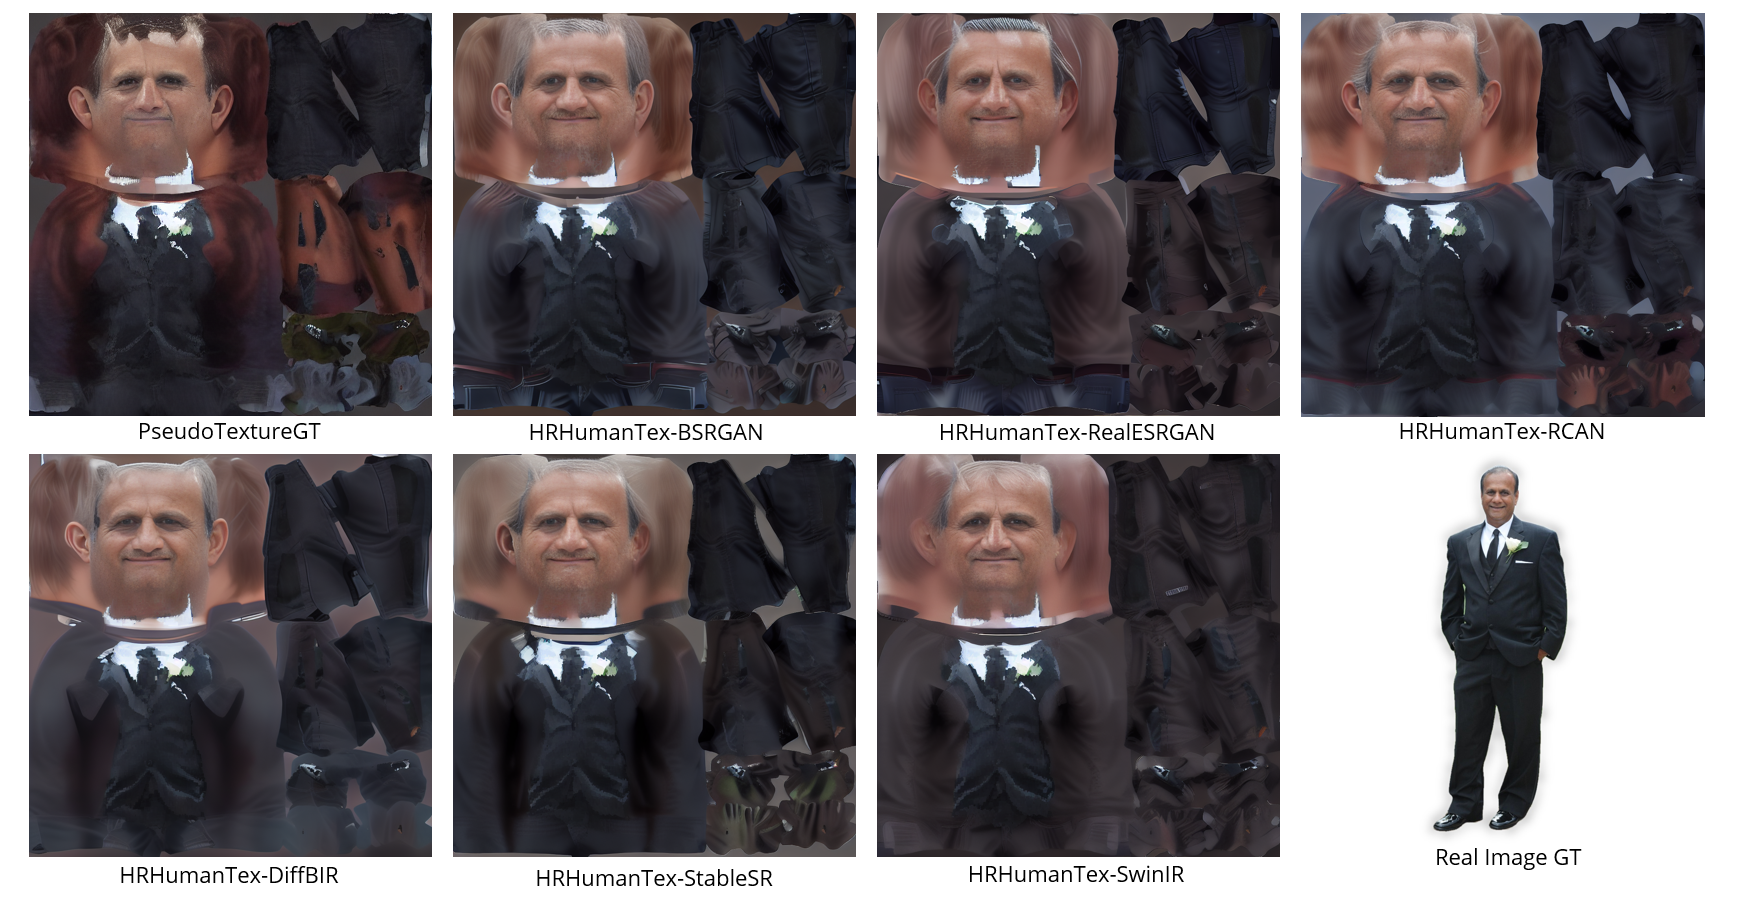
\includegraphics[width=1\textwidth]{fig/shhq1.png}
    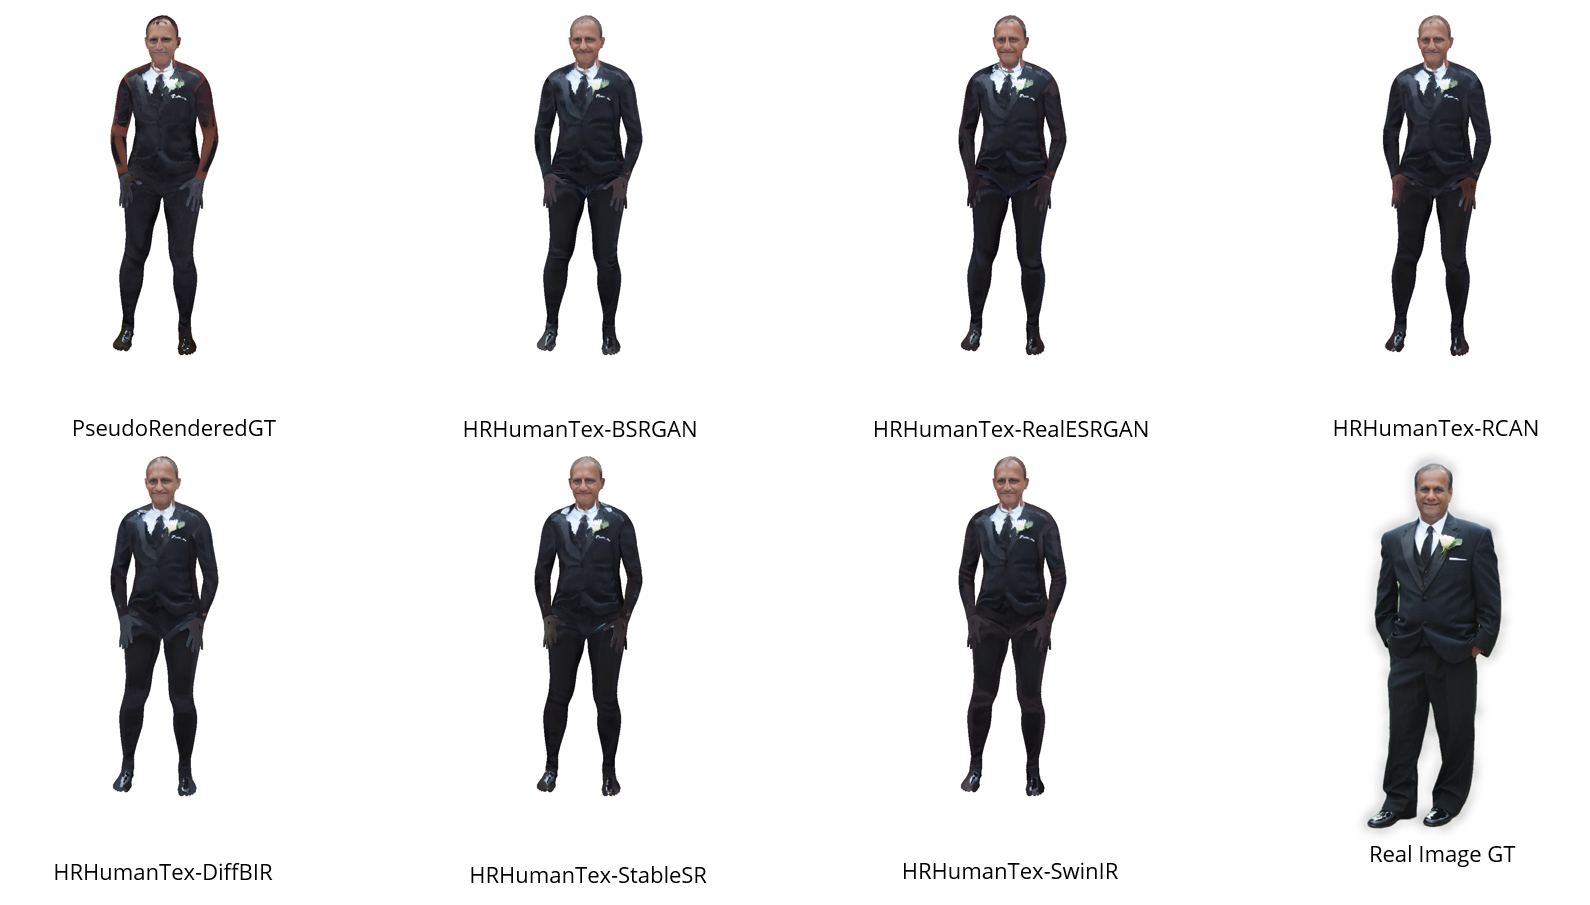
\includegraphics[width=1\textwidth]{fig/shhq7.png}
	\caption{Visual comparison of different inpainting models in UV space and rendered images, data sampled from dataset SHHQ-1.0 from~\cite{fu2022styleganhuman}.}
	\label{fig:shhqvisual}
\end{figure}


\begin{figure}[ht]
	\centering
	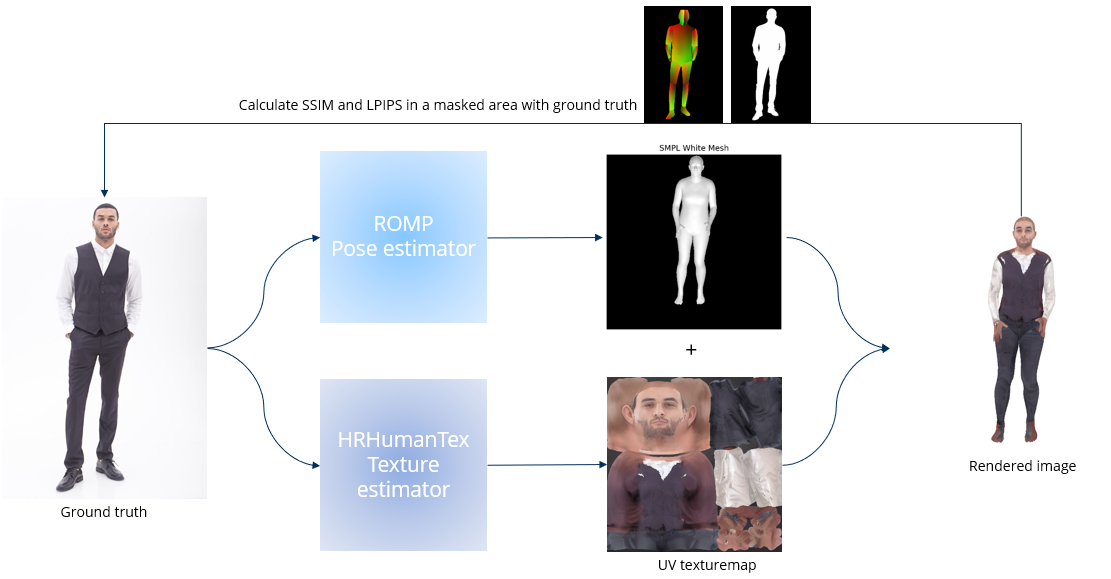
\includegraphics[width=0.85\textwidth]{fig/renderPGT.png}
	\caption{Construction of rendering based evaluation}
	\label{fig:inpainteval3}
\end{figure}

\paragraph{Step 3: Quantitative Analysis.}
I compare each predicted texture $\hat{T}^{(i)}$ with the pseudo-ground-truth $T_{\text{SRFormer}}$ using standard fidelity metrics:

\begin{itemize}
\item \textbf{PSNR}, \textbf{SSIM}, \textbf{LPIPS} and \textbf{FID} in UV space.
\item Rendered mesh views (by  PyTorch3D~\cite{ravi2020pytorch3d} and ROMP~\cite{ROMP}) and compare against real photo references.
\end{itemize}

To evaluate the perceptual quality of the predicted high-resolution UV texture maps, I conduct a rendering-based evaluation following a standardized 3D pipeline. This ensures that I assess texture fidelity not only in UV space but also in final rendered appearance under realistic lighting and geometry conditions. My implementation is based on PyTorch3D and includes the following steps:

\paragraph{UV Template Preparation.} 
I pre-load a standardized UV template using the official SMPL UV layout, parsed from an OBJ file. The following components are extracted once at startup:
\begin{itemize}
  \item \texttt{verts\_uvs}: Per-vertex UV coordinates.
  \item \texttt{faces\_verts}: Triangular face indices (vertices).
  \item \texttt{faces\_uvs}: UV indices corresponding to faces.
\end{itemize}

\paragraph{Mesh and Texture Assembly.}
For each test subject, I load the SMPL parameters (\texttt{betas}, \texttt{pose}, \texttt{global orient}) from a corresponding \texttt{.npz} file. I then forward the SMPL model to obtain the posed mesh:
\[
\mathbf{V} = \texttt{SMPL}(\boldsymbol{\beta}, \boldsymbol{\theta}, \boldsymbol{\gamma})
\]
Given the predicted UV texture image (from our inpainting network), I create a \texttt{TexturesUV} object and assemble a \texttt{Meshes} instance combining geometry and texture.
\paragraph{Camera and Lighting Configuration.}
To ensure consistent evaluation:
\begin{itemize}
  \item I use a fixed frontal camera view (\texttt{azimuth} = 180°).
  \item An orthographic camera model is used to avoid perspective distortion.
  \item Lighting is simplified to white ambient light without specular highlights.
\end{itemize}
The rendered image is corrected by vertical (\texttt{flipud}) and horizontal (\texttt{fliplr}) flipping to align with the GT projection orientation.

\paragraph{Masked Metric Computation.}
For fair evaluation, I apply a binary mask derived from:
\begin{itemize}
  \item \textbf{DensePose} output (from SMPL-based projection).
  \item Optional \textbf{segmentation silhouette} from SGHM.
\end{itemize}

The final metric mask is the logical AND of these two binary masks. Using this mask, I compute SSIM and LPIPS between the rendered image and ground-truth reference.

\paragraph{Metrics.} 
The following perceptual metrics are used:
\begin{itemize}
  \item \textbf{SSIM}: Computed using a window size of 7, \texttt{data\_range=1.0}, with channel-wise comparison.
  \item \textbf{LPIPS}: Computed using the pre-trained AlexNet backbone from the official LPIPS package.
\end{itemize}

 Figure~\ref{fig:inpainteval3} shows how I construct rendering-based evaluation. After I got the results of the pseudo ground truth evaluation, I calculated the other inpainting model's results and made a scatter plot~\ref{fig:inpainteval2} of rendering-based evaluation results. Figure~\ref{fig:shhqvisual} shows the visual detail comparison on different inpainting models in UV space and rendered images. More qualitative visual comparison will be presented in the Results chapter.

\paragraph{Conclusion of the period}
This three-stage evaluation allows me to not only choose the best SR model for direct upsampling, but also the one that produces the most useful 1024px training data for DreamBooth. While HRHumanTex-SwinIR achieve the best perceptual fidelity in UV space, its performance diverges under rendering evaluation. HRHumanTex-DiffBIR performs a high SSIM, indicating a consistent appearance after mapping to the 3D mesh. In contrast, HRHumanTex-SwinIR fails to preserve structure when rendered, implying a form of UV overfitting.

Interestingly, both HRHumanTex-Real-ESRGAN and HRHumanTex-DiffBIR report high SSIM after rendering, but their LPIPS scores remain elevated, suggesting that while geometric alignment is achieved, the perceptual realism suffers from over-smoothing or inconsistent textures. HRHumanTex-SwinIR and HRHumanTex-DiffBIR stand out with a balanced performance across both spaces, making them a stable and generalizable baseline for high-resolution human texture tasks.



\section{HRHumanTex Full Pipeline}

The High-Resolution Human Texture Estimation(HRHumanTex) pipeline extends SMPLitex by scaling the resolution and integrating super-resolution (SR) and high-fidelity inpainting into a unified pipeline. This section formalizes the pipeline and its evaluation in mathematical terms and outlines the integration strategy that yielded the final, high-resolution model. Figure~\ref{fig:hrhumentex} shows the overall pipeline of HRHumanTex.

\begin{figure}[ht]
	\centering
	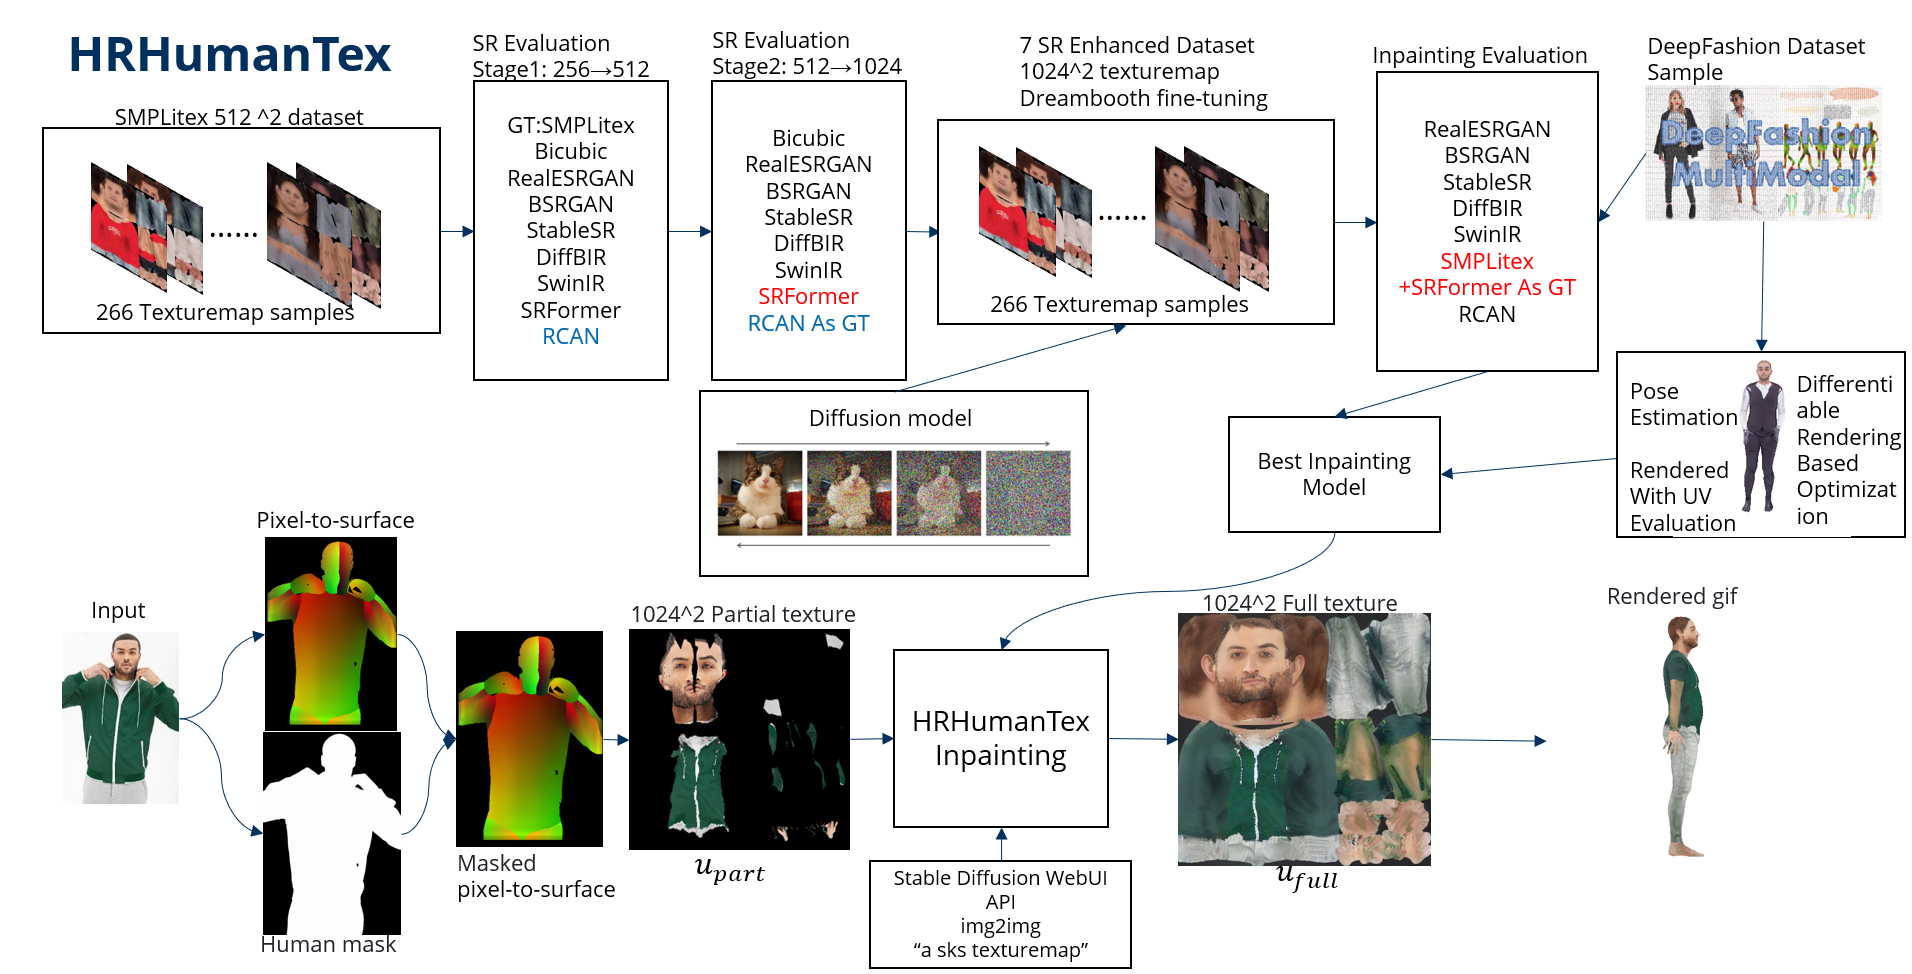
\includegraphics[width=1.0\textwidth]{fig/HRHumanTexpipeline.png}
	\caption{High Resolution Human Texture Estimation Pipeline}
	\label{fig:hrhumentex}
\end{figure}

\subsection{Pipeline Structure and Model Classes}

The full HRHumanTex pipeline consists of the following stages:

\begin{enumerate}
    \item \textbf{Stage 1 (Low-Resolution SR Evaluation):} Evaluate different SR models on 256$\rightarrow$512 upsampling using real 512px ground truth.
    \item \textbf{Stage 2 (High-Resolution SR Evaluation):} Use RCAN outputs as pseudo-ground truth to evaluate 512$\rightarrow$1024 performance of all SR models.
    \item \textbf{Stage 3 (Inpainting Evaluation):} Use SRFormer-upscaled textures as pseudo-ground truth, and compare different inpainting models trained on SR-upsampled datasets.
\end{enumerate}

\subsection{Mathematical Formulation of the Pipeline}

Let $\mathbf{u}_{\text{LR}}$ denote a low-resolution ($512\times512$) texture. Each SR model $\mathcal{F}_{\theta(i)}$ generates a high-resolution texture:

\begin{equation}
\mathbf{u}^{(i)}_{\text{HR}} = \mathcal{F}_{\theta(i)}(\mathbf{u}_{\text{LR}}), \quad i = 1, \dots, 7
\end{equation}

Next, for each input image, I extract a partial texture $\mathbf{u}_{\text{part}}$ using DensePose and SGHM, and provide this (along with its mask $\mathbf{m}$) to an inpainting model $\mathcal{D}_\phi$ to predict the full texture:

\begin{equation}
\hat{\mathbf{u}}_{\text{full}} = \mathcal{D}_\phi(\mathbf{u}_{\text{part}}, \mathbf{m})
\end{equation}

Training minimizes the following conditional log-likelihood:

\begin{equation}
\max_{\phi} \; \mathbb{E}_{\mathbf{u}_{\text{part}}, \mathbf{m}, \mathbf{u}_{\text{full}}} 
\left[ \log p_\phi\left( \mathbf{u}_{\text{full}} \mid \mathbf{u}_{\text{part}}, \mathbf{m} \right) \right]
\end{equation}


This process is illustrated in Algorithm~\ref{alg:full_pipeline_eval}.

\begin{algorithm}[t]
\caption{Three-Stage Evaluation for HRHumanTex}
\label{alg:full_pipeline_eval}
\SetAlgoNlRelativeSize{0}
\SetKwComment{Comment}{$\triangleright$\ }{}
\DontPrintSemicolon

\KwIn{SMPLitex dataset $\mathcal{T}$, 7 SR models $\{\mathcal{F}_{\theta(i)}\}$, input images $\mathcal{X}$}

\vspace{4pt}
\textbf{Stage 1:} For each $\mathbf{u} \in \mathcal{T}$, create 256px version, apply $\mathcal{F}_{\theta(i)}$, and evaluate against GT (512px).

\vspace{4pt}
\textbf{Stage 2:} For each $\mathbf{u} \in \mathcal{T}$, use RCAN to produce pseudo-GT at 1024px. Compare other SR outputs to this.

\vspace{4pt}
\textbf{Stage 3:} For each image $x \in \mathcal{X}$:

\Indp
\begin{itemize}
\item Extract partial texture $\mathbf{u}_{\text{part}}$ and mask $\mathbf{m}$ using DensePose + SGHM
\item For each model $\mathcal{D}^{(i)}_\phi$ trained on SR-$i$ data, predict:
$$\hat{\mathbf{u}}_{\text{full}}^{(i)} = \mathcal{D}^{(i)}_\phi(\mathbf{u}_{\text{part}}, \mathbf{m})$$
\item Compare each prediction $\hat{\mathbf{u}}_{\text{full}}^{(i)}$ to SRFormer pseudo-GT and render-based reference using LPIPS, SSIM, PSNR, and UV fidelity.
\end{itemize}
\Indm

\KwOut{Best SR source for inpainting model training.}
\end{algorithm}


\subsection{Evaluation Metrics}

To evaluate the quality of the generated textures, I use several standard image fidelity metrics, as well as a task-specific UV-space measure.

\paragraph{PSNR.} The Peak Signal-to-Noise Ratio (PSNR) measures per-pixel reconstruction quality. Given predicted texture $I$ and ground truth $I_{\text{gt}}$, I compute mean squared error (MSE), and then:

\begin{equation}
\text{PSNR} = 10 \log_{10} \left( \frac{L^2}{\text{MSE}} \right)
\end{equation}

where $L=1$ for normalized images. Higher PSNR indicates lower distortion.

\paragraph{SSIM.} The Structural Similarity Index (SSIM) compares luminance, contrast, and structure between images:

\begin{equation}
\text{SSIM}(I, I_{\text{gt}}) = \frac{(2\mu_I \mu_{I_{\text{gt}}} + C_1)(2\sigma_{I I_{\text{gt}}} + C_2)}{(\mu_I^2 + \mu_{I_{\text{gt}}}^2 + C_1)(\sigma_I^2 + \sigma_{I_{\text{gt}}}^2 + C_2)}
\end{equation}

where $\mu$, $\sigma$ are local means and variances. I report SSIM as it reflects structure preservation in textures.

\paragraph{LPIPS.} I use LPIPS to evaluate perceptual similarity between textures. It compares deep features extracted from a pretrained VGG model:

\begin{equation}
\text{LPIPS}(I, I_{\text{gt}}) = \sum_l w_l \| \hat{f}_l(I) - \hat{f}_l(I_{\text{gt}}) \|^2
\end{equation}

Lower LPIPS implies the result is perceptually closer to the target.

\paragraph{FID.} The Fréchet Inception Distance (FID) measures how close the feature distributions of generated textures and real textures are:

\begin{equation}
\text{FID} = \| \mu - \mu_{\text{gt}} \|^2 + \text{Tr}( \Sigma + \Sigma_{\text{gt}} - 2 (\Sigma \Sigma_{\text{gt}})^{1/2} )
\end{equation}


\subsection{Implementation Details and Challenges}

\paragraph{Overview.} I build upon the SMPLitex framework but replace its original low-resolution (512×512) inpainting pipeline with a high-resolution 1024×1024 diffusion-based system. The goal is to generate complete UV textures from partial inputs at $1024^2$ resolution. To achieve this, I first enhance the resolution of training textures using various super-resolution (SR) models, then train diffusion-based inpainting models using DreamBooth. Finally, I compare inpainting quality across different HRHumanTex variants and dataset scales.

\paragraph{Training Dataset Scaling.}
I use the 266-texture SMPLitex dataset (originally at $512\times512$ resolution) as the base for training. To enable 1024-resolution inpainting, I apply Real-ESRGAN to upscale the textures to $1024\times1024$. To understand how dataset size affects inpainting performance, I create four subsets of increasing size: 20, 50, 100, and all 266 textures. I train separate DreamBooth models on each. When testing, I find that:

\begin{itemize}
    \item Training on just 20 textures leads to poor generalization, with only central body regions (e.g., face, torso) being reliably completed.
    \item At 50 textures, side limbs and color transitions become more coherent.
    \item At 100 textures, the model learns to complete nearly all body regions at $1024^2$ resolution.
    \item Full 266-texture training yields the most consistent and high-fidelity textures.
\end{itemize}

This confirms that at least 100 high-res samples are needed for effective 1024px completion.

\paragraph{Super-Resolution Model Comparison.}
To prepare the 1024px datasets for HRHumanTex, I perform a two-stage super-resolution evaluation:

\begin{itemize}
    \item For the $256 \rightarrow 512$ setting, I downsample the original textures to $256\times256$ and evaluate 8 SR methods (RCAN, BSRGAN, Real-ESRGAN, SwinIR, DiffBIR, SRFormer, StableSR, and Bicubic). I compare their outputs to the original 512px ground truth using PSNR, SSIM, and LPIPS. RCAN performs best in this stage.
    \item Since no real 1024px ground truth is available, I use RCAN's output as a pseudo-ground truth for the $512 \rightarrow 1024$ stage. I then apply each SR model to upscale 512px inputs and evaluate them against the RCAN-based pseudo-GT. In this comparison, SRFormer performs best.
\end{itemize}

This motivates the use of RCAN for generating high-quality pseudo-GT data, and SRFormer as an effective 512→1024 super-resolver.

\paragraph{DreamBooth Training Configuration.}
I train all HRHumanTex models using the following settings:

\begin{itemize}
    \item \textbf{Model:} Stable Diffusion v1.5 inpainting variant.
    \item \textbf{Training resolution:} $1024\times1024$.
    \item \textbf{Prompt:} ``a sks texturemap'' (instance), ``a texturemap'' (class).
    \item \textbf{GPU:} NVIDIA RTX 3090 (24\,GB).
    \item \textbf{Batch size:} 1; Gradient accumulation: 8 steps.
    \item \textbf{Optimizer:} 8-bit AdamW, learning rate $1 \times 10^{-6}$.
    \item \textbf{Steps:} 2000 (with checkpointing every 500).
    \item \textbf{Training time:} approx. 6–7 hours per model.
\end{itemize}

I use the following command template:

\begin{lstlisting}[language=bash]
accelerate launch --mixed_precision="fp16" train_dreambooth.py \
  --pretrained_model_name_or_path=$MODEL_NAME \
  --instance_data_dir=$INSTANCE_DIR \
  --output_dir=$OUTPUT_DIR \
  --class_data_dir=$CLASS_DIR \
  --with_prior_preservation --prior_loss_weight=1.0 \
  --instance_prompt="a sks texturemap" \
  --class_prompt="a texturemap" \
  --resolution=1024 \
  --train_batch_size=1 \
  --gradient_accumulation_steps=8 \
  --gradient_checkpointing \
  --learning_rate=1e-6 \
  --lr_scheduler="constant" \
  --lr_warmup_steps=0 \
  --num_class_images=10 \
  --max_train_steps=2000 \
  --checkpointing_steps=500 \
  --train_text_encoder \
  --use_8bit_adam
\end{lstlisting}

\paragraph{HRHumanTex Variants.}
I train one HRHumanTex model for each of the seven SR models mentioned earlier (plus Bicubic), using the full set of 266 textures. Each variant is ~4GB in size. Table~\ref{tab:hrhumantex-variants} summarizes training conditions.

\begin{table}[h]
\centering
\caption{Training configuration of HRHumanTex variants}
\label{tab:hrhumantex-variants}
\begin{tabular}{lccc}
\toprule
Model Variant & Data Size & SR Method & Training Time \\
\midrule
SMPLitex-20         & 20 (Real-ESRGAN) & -          & $\sim$6 h \\
SMPLitex-50         & 50 (Real-ESRGAN) & -          & $\sim$6 h \\
SMPLitex-100        & 100 (Real-ESRGAN) & -         & $\sim$6 h \\
HRHumanTex-RCAN     & 266 & RCAN       & $\sim$7 h \\
HRHumanTex-BSRGAN   & 266 & BSRGAN     & $\sim$7 h \\
HRHumanTex-RealESRGAN & 266 & Real-ESRGAN & $\sim$7 h \\
HRHumanTex-SwinIR   & 266 & SwinIR     & $\sim$7 h \\
HRHumanTex-DiffBIR  & 266 & DiffBIR    & $\sim$7 h \\
HRHumanTex-SRFormer & 266 & SRFormer   & $\sim$7 h \\
HRHumanTex-StableSR & 266 & StableSR   & $\sim$7 h \\
\bottomrule
\end{tabular}
\end{table}

\paragraph{Testing and Evaluation.}
I test the inpainting quality of each model using 50 challenging samples from the DeepFashion dataset. These include diverse poses, garments, skin tones, and occlusion patterns. For each image:

\begin{enumerate}
    \item Extract partial textures via DensePose and SGHM.
    \item Apply each HRHumanTex model to complete the full texture.
    \item Render the result on the SMPL mesh.
    \item Compare rendered images against the original photo using LPIPS, SSIM.
\end{enumerate}

\paragraph{Challenges.}
Key challenges during implementation include:

\begin{itemize}
    \item \textbf{Hallucinated Faces:} Training directly at 1024px using the base Stable Diffusion inpainting model causes facial artifacts in non-face UV areas. Fine-tuning with more samples resolves this.
    \item \textbf{Sample Efficiency:} At least 100 high-res examples are required to enable reliable learning of complete texture structure.
    \item \textbf{Memory Bottlenecks:} 1024px DreamBooth training is GPU-intensive. I use 8-bit Adam, gradient checkpointing, and reduce UNet depth where necessary.
    \item \textbf{Perceptual Tradeoff:} GAN-based SR models yield sharper textures that score worse on LPIPS. I provide both ``fidelity'' and ``photorealistic'' modes for downstream applications.
\end{itemize}

\subsection{Rendering-Based Evaluation Implementation Details}

To evaluate the texture quality in image space after projection onto the 3D body, I follow a structured rendering-based evaluation pipeline using PyTorch3D and standard perceptual metrics.

\subsubsection{Pipeline Overview}

\textbf{(1) UV Template Loading.}
A static SMPL UV template is loaded once at startup via:
\begin{lstlisting}[language=Python]
verts_uvs, faces_uvs_idx, faces_verts_idx = load_obj(uv_obj)
\end{lstlisting}
This provides the UV coordinates and mesh face indices required for UV-based texturing.

\textbf{(2) SMPL Forward Pass.}
Given the estimated pose parameters (\texttt{body\_pose}, \texttt{global\_orient}) and shape parameters (\texttt{betas}), we compute the posed 3D vertices:
\begin{lstlisting}[language=Python]
smpl_model = SMPL(...).to(device)
output = smpl_model(betas, body_pose, global_orient, return_verts=True)
verts = output.vertices[0]
\end{lstlisting}

\textbf{(3) Texture-Mesh Assembly.}
The predicted UV texture is wrapped onto the mesh using:
\begin{lstlisting}[language=Python]
textures = TexturesUV(maps=tex_np, faces_uvs=faces_uvs, verts_uvs=verts_uvs)
mesh = Meshes(verts=[verts], faces=[faces_verts_idx], textures=textures)
\end{lstlisting}

\textbf{(4) Camera Correction.}
I observed that initial renderings were flipped and back-facing due to SMPL coordinate conventions. To address this, we fixed the azimuth to $180^\circ$, and additionally flipped the rendered output along both axes:
\begin{lstlisting}[language=Python]
img = np.flipud(np.fliplr(rendered_img))
\end{lstlisting}

\textbf{(5) Metric Computation.}
Two perceptual metrics were used:
\begin{itemize}
    \item \textbf{SSIM}: Computed with \texttt{skimage.metrics.ssim}, ensuring floating-point inputs and specifying \texttt{data\_range=1.0}.
    \item \textbf{LPIPS}: Using the pretrained \texttt{lpips.LPIPS(net='alex')} model. Input images are normalized to $[-1, 1]$ and passed as tensors.
\end{itemize}

\textbf{(6) Result Handling.}
Each successfully rendered result is saved for visualization and analysis. Failures (e.g., due to invalid geometry or pose) are logged along with debug visualizations.

\subsubsection{Implementation Challenges and Solutions}

\begin{itemize}
    \item \textbf{Camera Orientation}: SMPL-rendered bodies appeared flipped or rotated. Resolved with a fixed view transform and image flips.
    \item \textbf{Device/Dtype Consistency}: To prevent silent runtime failures, all tensors were explicitly cast to \texttt{float()} and moved to the correct \texttt{device}.
    \item \textbf{SSIM Range Errors}: SSIM computations on float inputs require explicit \texttt{data\_range}; failure to do so raises exceptions.
    \item \textbf{Inconsistent \texttt{.npz} Structures}: Some intermediate files store data as nested \texttt{'results'} dicts, while others use flat key-value pairs. We handle both formats robustly:
    \begin{lstlisting}[language=Python]
data_npz = np.load(npz_path, allow_pickle=True)
data = data_npz['results'].item() if 'results' in data_npz.files else dict(data_npz)
    \end{lstlisting}
\end{itemize}


\subsection{Ablation Study B: DreamBooth Hyperparameters}

To understand the effect of key hyperparameters in DreamBooth training for UV texture inpainting, I conducted a series of controlled experiments by modifying the training settings on top of the HRHumanTex pipeline. The goal was to investigate how different configurations affect the model’s ability to hallucinate plausible high-resolution textures at 1024$\times$1024.

\paragraph{Diffusion Backbone Version.}
I compared Stable Diffusion v1.4 and v1.5 inpainting variants. While v1.4 is the original version used in SMPLitex, v1.5 contains improved VAE encoding and slightly better noise scheduling. I found that v1.5 led to cleaner textures with fewer artifacts, especially in challenging occlusion regions, and thus I used it for all HRHumanTex models.

\paragraph{Training Steps.}
I increased the training steps from 1500 (as used in SMPLitex) to 2000 to accommodate the higher-resolution training. This gave the model additional capacity to refine the global structure and fill in peripheral texture details. Without the increase, 1024px outputs often lacked coherence at the body edges.

\paragraph{Resolution.}
A core difference from SMPLitex is the shift from $512\times512$ to $1024\times1024$ texture generation. While this improved output detail significantly, it also introduced GPU memory constraints. To support this, I had to adjust the batch strategy.

\paragraph{Gradient Accumulation.}
To simulate a larger effective batch size without exceeding VRAM limits, I increased the gradient accumulation steps from 2 (baseline) to 8. This provided more stable gradients during DreamBooth training and helped reduce artifacts, especially in background-foreground transitions.

\paragraph{Optimization Strategy.}
I used 8-bit AdamW optimizer and enabled gradient checkpointing in all models. These settings were essential for fitting 1024px DreamBooth training into a 24GB RTX3090. Disabling either often resulted in out-of-memory (OOM) errors.

\paragraph{Summary.}
The final configuration for all HRHumanTex variants used Stable Diffusion v1.5, 2000 training steps, $1024\times1024$ resolution, 8-step gradient accumulation, 8-bit AdamW, and full encoder fine-tuning. These settings collectively allowed high-resolution DreamBooth to converge on detailed, artifact-free texture completions.

\subsection{Rendering-Based Texture Optimization (Exploratory)}
\label{sec:render_opt}

To further explore the potential of refining UV textures beyond initial estimation or inpainting, I conducted an experiment based on differentiable rendering~\cite{ravi2020pytorch3d}. The goal of this exploratory setup is to directly optimize a UV texture map such that, when rendered on a 3D mesh using SMPL geometry, the output image aligns closely with a given reference view.

\paragraph{Motivation.}  
While HRHumanTex models can successfully estimate complete UV textures from a single image, their outputs often contain artifacts, such as inconsistent shading or blurry regions. Instead of retraining an entire network, I experiment with a more lightweight approach: treating the UV texture as a learnable tensor and optimizing it directly in pixel space, using rendered images as the bridge between surface and appearance.

\paragraph{Setup.}  
Starting from an initial 1024$\times$1024 UV texture by HRHumanTex, I render it onto a SMPL mesh under a known camera pose extracted from an associated .npz file. The rendered image is then compared to a ground-truth reference image. The UV texture itself is defined as a floating-point tensor with gradients enabled (`requires\_grad=True`), and updated using backpropagation.

\paragraph{Loss Functions.}  
I use a weighted combination of three loss terms to guide the optimization:
\begin{itemize}
    \item \textbf{L2 loss}: per-pixel difference between the rendered image and the reference.
    \item \textbf{LPIPS loss}: a learned perceptual similarity measure.
    \item \textbf{VGG perceptual loss}~\cite{johnson2016perceptuallossesrealtimestyle}: early-layer differences from a pretrained VGG16 network.
\end{itemize}

The total loss is defined as:
\begin{equation}
\mathcal{L} = \mathcal{L}_{\text{L2}} + 0.1 \cdot \mathcal{L}_{\text{LPIPS}} + 0.01 \cdot \mathcal{L}_{\text{VGG}}.
\end{equation}

To avoid background influence, I compute all losses only over the visible human region, using a silhouette mask derived from mesh rasterization.

\paragraph{Implementation Details.}  
This experiment is implemented in PyTorch using PyTorch3D for rendering. I use a fixed orthographic camera based on the predicted SMPL pose and translation. The optimization is performed using Adam with a learning rate of 0.01 for 1000 steps. Every 100 iterations, I save the intermediate texture and rendered image for visual inspection. The learning rate is set as 1e-2, because the gradient is large enough, the update amount is sufficient, the loss decreases quickly and it is not easy to fall into the flat area.

The entire pipeline runs on a single RTX 3090 GPU, and takes under 10 minutes per texture. To correct coordinate mismatches, I vertically and horizontally flip the rendered image before comparison.

\begin{figure}[ht]
	\centering
	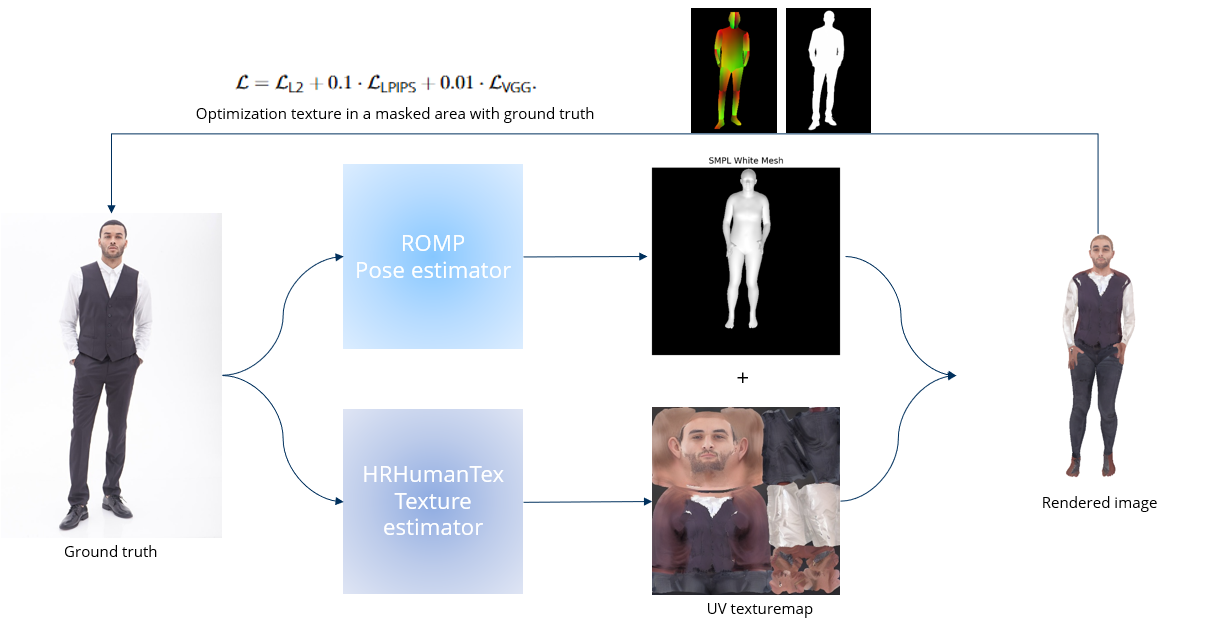
\includegraphics[width=0.9\textwidth]{fig/optimizetex.png}
	\caption{Differentiable Rendering Based Texture Optimization Pipeline}
	\label{fig:dr_tex}
\end{figure}

\begin{figure}[ht]
	\centering
	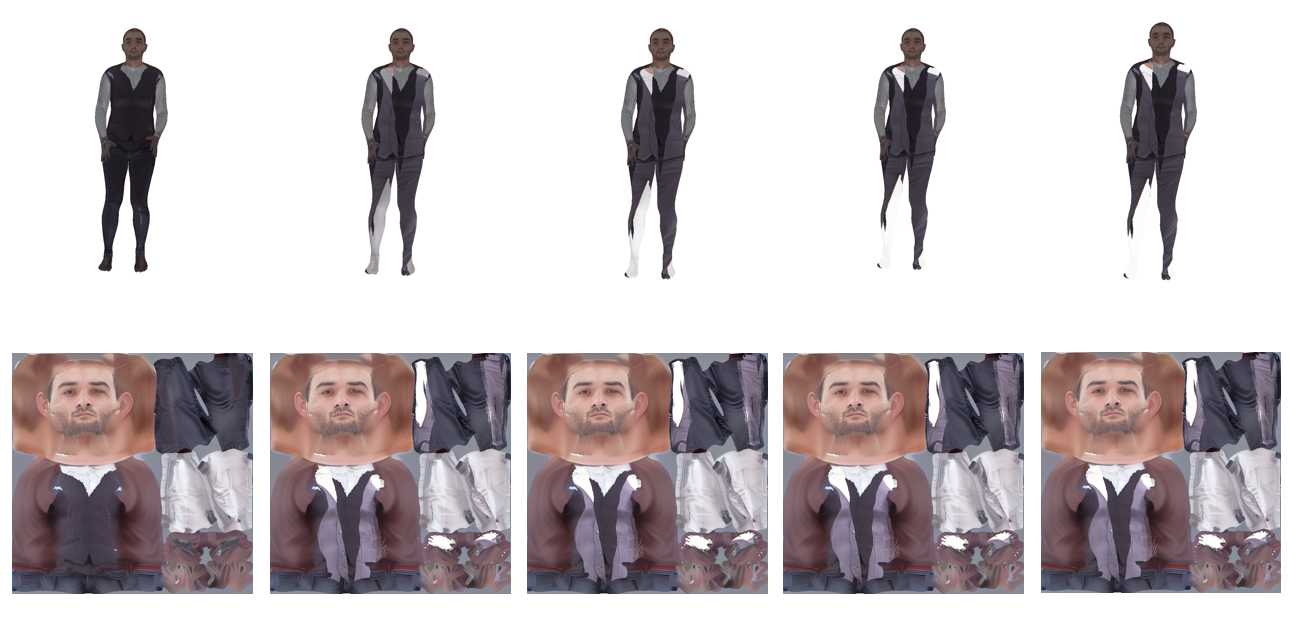
\includegraphics[width=0.9\textwidth]{fig/iterativetex.png}
	\caption{Iterative texture optimization process, from left (initial) to right (final).}
	\label{fig:ite_tex}
\end{figure}

\paragraph{Observations.}  
Even with a single-view setup, I observe that the texture becomes visually sharper and more aligned with the reference over the course of optimization. In particular, I find that the model tends to recover mid-frequency patterns such as cloth folds and contour shading that were missing in the initial HRHumanTex estimation pipeline. However, the improvements are not so much in the UV space. Figure~\ref{fig:dr_tex} shows the architecture of this texture optimization pipeline. And Figure~\ref{fig:ite_tex} shows this exploratory experiment's results.

This exploratory experiment suggests that differentiable rendering can serve as a lightweight post-processing strategy to fine-tune UV textures, especially when paired with high-quality reference images. In future work, I plan to extend this approach to multi-view optimization and region-aware masking using DensePose or semantic segmentation maps. More experiments results shows below~\ref{fig:ite_tex2} and ~\ref{fig:ite_tex3}.

\begin{figure}[ht]
	\centering
	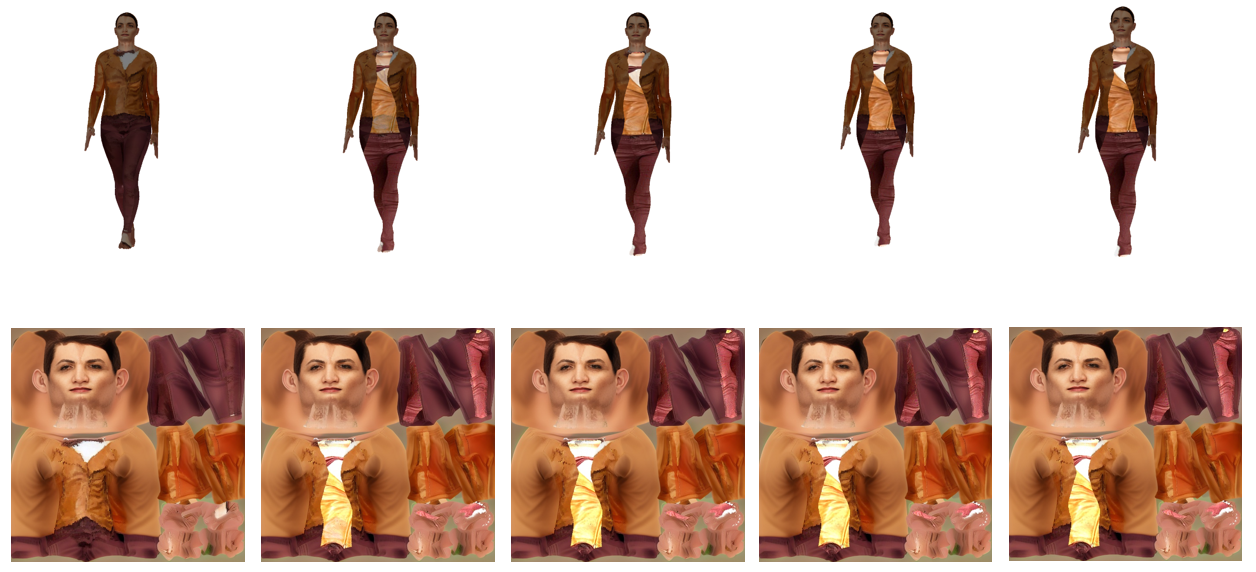
\includegraphics[width=0.9\textwidth]{fig/dro1}
    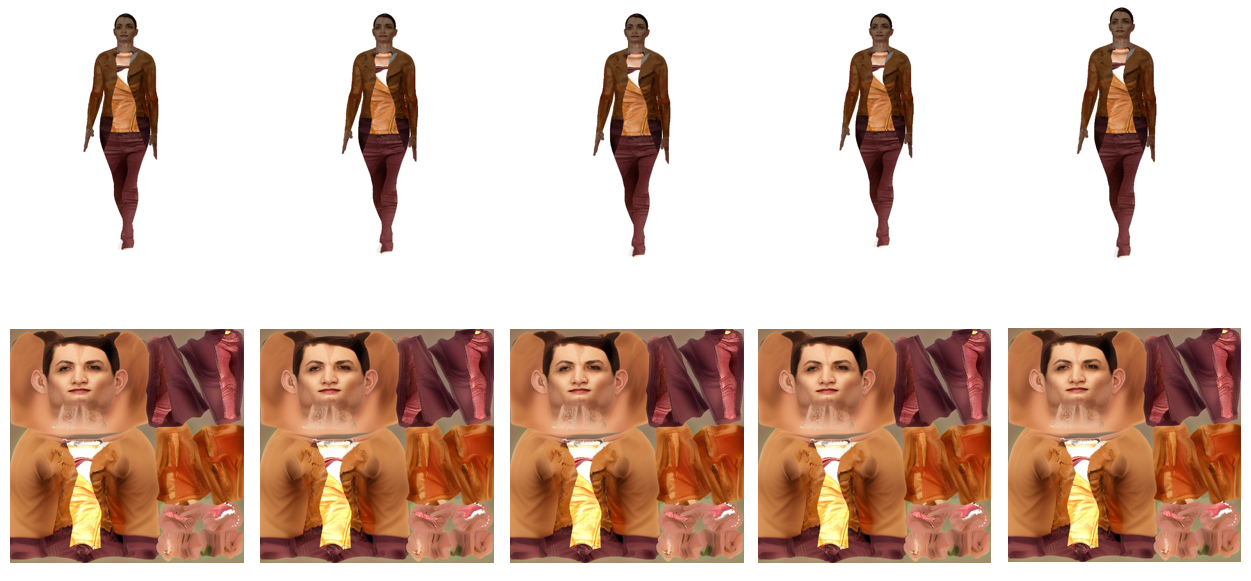
\includegraphics[width=0.9\textwidth]{fig/dro2}
	\caption{Iterative texture optimization process with more middle results, from left (initial) to right (final).}
	\label{fig:ite_tex2}
\end{figure}

\begin{figure}[ht]
	\centering
	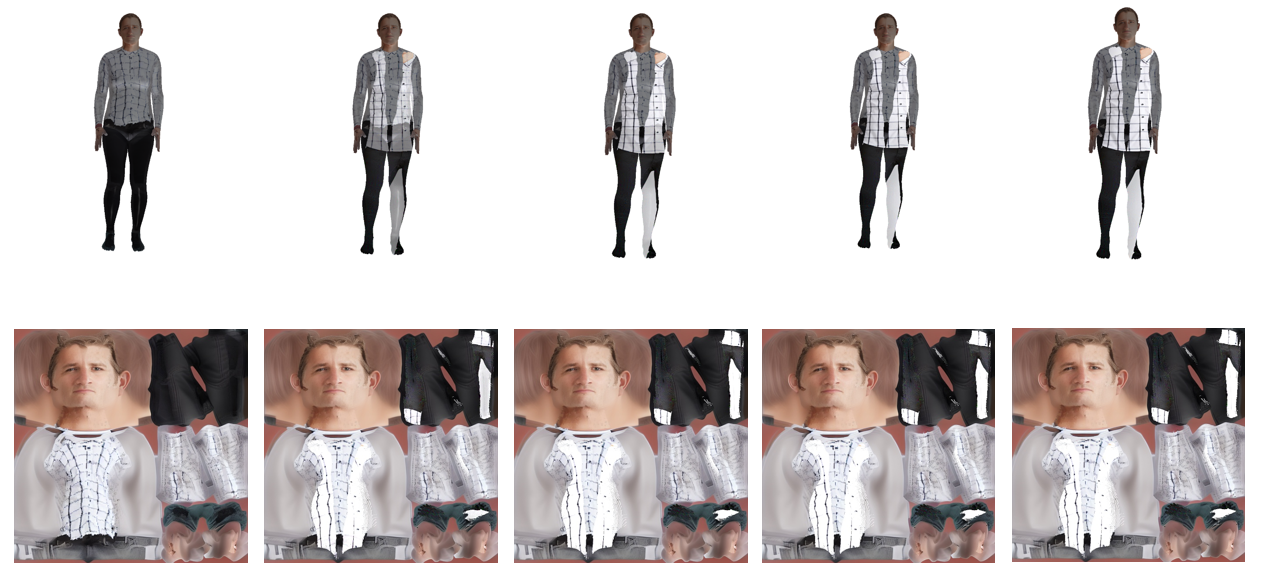
\includegraphics[width=0.9\textwidth]{fig/dro3.png}
    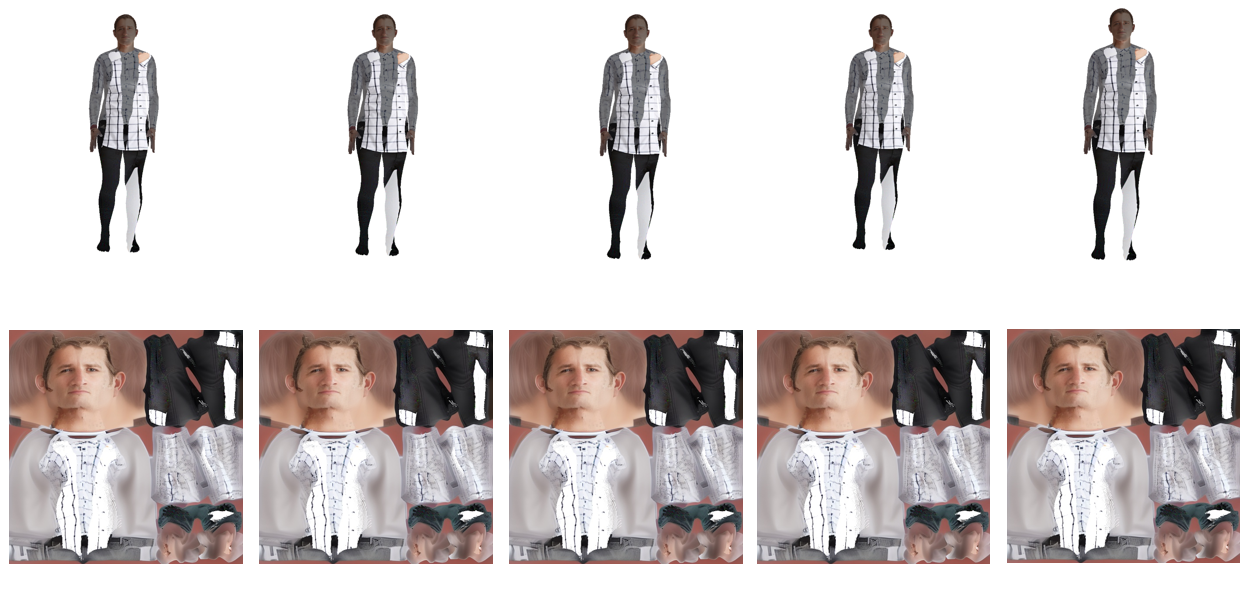
\includegraphics[width=0.9\textwidth]{fig/dro4.png}
	\caption{Iterative texture optimization process with more middle results, from left (initial) to right (final).}
	\label{fig:ite_tex3}
\end{figure}

According to these results, a more accurate Pose Estimator or image dataset with distinct pose and camera parameters will performance better at this texture quality optimization module.